% -------------------------------------------------------------------------------
% Establish page structure & font.
\documentclass[12pt]{report}

\usepackage[total={6.5in, 9in},
	left=1in,
	right=1in,
	top=1in,
	bottom=1in,]{geometry} % Page structure

\usepackage{graphicx} % Required for inserting images
\graphicspath{{../.images}} % Any additional images I use (BCU logo, etc) are from here.

\usepackage[utf8]{inputenc} % UTF-8 encoding
\usepackage[T1]{fontenc} % T1 font
\usepackage{float}  % Allows for floats to be positioned using [H], which correctly
                    % positions them relative to their location within my LaTeX code.
\usepackage{subcaption}
\usepackage{csquotes}

% -------------------------------------------------------------------------------
% Declare biblatex with custom Harvard BCU styling for referencing.
\usepackage[
    useprefix=true,
    maxcitenames=3,
    maxbibnames=99,
    style=authoryear,
    dashed=false, 
    natbib=true,
    url=false,
    backend=biber
]{biblatex}

\usepackage[british]{babel}

% Additional styling options to ensure Harvard referencing format.
\renewbibmacro*{volume+number+eid}{
    \printfield{volume}
    \setunit*{\addnbspace}
    \printfield{number}
    \setunit{\addcomma\space}
    \printfield{eid}}
\DeclareFieldFormat[article]{number}{\mkbibparens{#1}}

% Declaring all three bibs.
\addbibresource{Proposal.bib}
\addbibresource{LitReview.bib}
\addbibresource{Dissertation.bib}


% -------------------------------------------------------------------------------
% To prevent "Chapter N" display for each chapter
\usepackage[compact]{titlesec}
\usepackage{wasysym}
\usepackage{import}

\titlespacing*{\chapter}{0pt}{-2cm}{0.5cm}
\titleformat{\chapter}[display]
{\normalfont\bfseries}{}{0pt}{\Huge}

% -------------------------------------------------------------------------------
% Custom macro to make an un-numbered footnote.

\newcommand\blfootnote[1]{
    \begingroup
    \renewcommand\thefootnote{}\footnote{#1}
    \addtocounter{footnote}{-1}
    \endgroup
}

% -------------------------------------------------------------------------------
% Fancy headers; used to show my name, BCU logo and current chapter for the page.
\usepackage{fancyhdr}
\usepackage{calc}
\pagestyle{fancy}

\setlength\headheight{37pt} % Set custom header height to fit the image.

\renewcommand{\chaptermark}[1]{%
    \markboth{#1}{}} % Include chapter name.


% Lewis Higgins - ID 22133848           [BCU LOGO]                [CHAPTER NAME]
\lhead{Lewis Higgins - ID 22133848~~~~~~~~~~~~~~~
\includegraphics[width=1.75cm]{BCU}}
\fancyhead[R]{\leftmark}

% ------------------------------------------------------------------------------
% Used to add PDF hyperlinks for figures and the contents page.

\usepackage{hyperref}

\hypersetup{
    colorlinks=true,
    linkcolor=black,
    filecolor=magenta,
    urlcolor=blue,
    citecolor=black,
}

% ------------------------------------------------------------------------------
\usepackage{xcolor} 
\usepackage{colortbl}
\usepackage{longtable}
\usepackage{amssymb}
\usepackage{pdflscape}
% ------------------------------------------------------------------------------
\usepackage{tcolorbox}
\newcommand{\para}{\vspace{7pt}\noindent}
% -------------------------------------------------------------------------------

\title{CMP6200 Individual Undergraduate Project}
\author{Lewis Higgins}
\date{September 2024 – May 2025}

\begin{document}

\makeatletter
\begin{titlepage}
    
\includegraphics[width=0.3\linewidth]{BCUWide.jpg}\\[4ex]
    \vspace{1cm}
    \begin{center}
        {\huge \bfseries  CMP6200}\\[2ex]
        {\huge \bfseries  Individual Undergraduate Project}\\[2ex]
        {\huge \bfseries 2024 – 2025}\\[16ex]
        {\huge \bfseries University Artificially Intelligent Assistant}\\[6ex]
        
\includegraphics[width=0.1\linewidth]{Symbol.png}\\[40ex]
        Course: Computer \& Data Science\\
        Student Name: Lewis Higgins\\
        Student Number: 22133848\\
        Supervisor Name: Dr. Atif Azad\\
        Word count: 10,182
    \end{center}
\end{titlepage}
\makeatother
\thispagestyle{empty}
\newpage

\begin{abstract}
    Artificial intelligence (AI), natural language processing (NLP) and large language models (LLMs) are
    rapidly developing technologies, seeing constant advancements at a frequent basis.
    This project aims to leverage these new advancements, specifically in LLMs, to create a digital assistant 
    to help new students of Birmingham City University get acquainted to their new environment. This is accomplished 
    through the development of a chatbot web application which uses Retrieval-Augmented Generation (RAG) with 
    OpenAI's gpt-4o-mini LLM on an embedded vector database of university information. The development process 
    is thoroughly explored, with key elements of the chatbot's code being discussed in detail.
    The produced chatbot performs well, achieving 80\% answer correctness on a dataset of testing questions
    evaluated using DeepEval's GEval metric with a gpt-4o LLM and manual verification.
\end{abstract}

\setcounter{page}{-4}

\chapter*{Acknowledgements}
\thispagestyle{empty}
I would like to primarily acknowledge my project supervisor, Dr. Atif Azad, as having a major positive 
influence throughout the development of this project. His expertise and advice had a significant 
effect throughout the entire project's development and report writing, and both would be of substantially 
lower quality were it not for his guidance.

\para Additionally, I would like to acknowledge my father, who continually motivated me to produce high-quality 
work throughout a deeply challenging year. Without the support of both of these people, this project 
would not have been feasible, and for this I thank them both greatly.


\chapter*{Glossary}
\thispagestyle{empty}
\begin{table}[H]
    \begin{tabular}{|p{0.2\linewidth}|p{0.74\linewidth}|}
        \hline
        \cellcolor{blue!25}Terminology & \cellcolor{blue!25}Description\\
        \hline 

        AI & A field of computing dedicated to allowing computers to simulate human
        learning by training them on large amounts of data so that they can recognise patterns to classify or 
        predict unknown data. AI can only be as good as the data it is trained upon ("Garbage in, garbage out"), and could
        become biased if it is fed too much data of a certain type.\\

        % \hline

        % Generative AI & AI dedicated to the generation of content rather than prediction or 
        % classification. It is possible for generative AI to produce text, images and 
        % more recently, even video and sound. & LLMs, Tokens, Embedding \\

        \hline

        Natural Language Processing \newline (NLP) & NLP refers to the use of machine learning to encode and 
        process text to understand it similarly to humans, which can be used to allow direct 
        two-way conversation between users and computers.\\

        \hline
        
        LLMs & Large Language Models are a type of machine learning model dedicated to the recognition and generation of text.
        As suggested by their name, they are trained on enormous amounts of text data, which allows them 
        to have active conversations with users. There are many different LLMs, and as their size and 
        complexity increases, so too does the necessary processing power. 
        \\
        \hline 

        Retrieval-Augmented Generation \newline (RAG) & The optimisation of the generated text output of an LLM, incorporating
        an external data source to enhance its contextual knowledge and the subject relevancy of its outputs. \\

        \hline
        Chatbot \newline Conversational Agent & Software that simulates a natural conversation between the 
        computer and end user. Many chatbots, including the one to be produced in this project, utilise recent
        developments such as Generative AI and natural language processing (NLP) to interpret and respond to user queries.
        \autocite{IBMChatbotDef}\\

        % \hline

        % User Experience (UX) & The end user's overall experience of using a system, such as its ease of use and 
        % whether it is enjoyable to use. In the context of this project, it will refer to the user's 
        % ability to smoothly converse with the chatbot and how human-like it is. 
        % & Conversational design, usability, accessibility, human-computer interaction

        % \\

        \hline 

    \end{tabular}
    % \caption{The themes and keywords used in the literature search.}
    % \label{tab:Glossary}
\end{table}

\tableofcontents
\thispagestyle{empty}

% ? Hides the page number on the contents page itself.
\addtocontents{toc}{\protect\thispagestyle{empty}}


\footnotesize \listoffigures
\thispagestyle{empty}

\normalsize
\thispagestyle{empty}

% It's likely that this will be an obscenely long LaTeX file. Therefore, it's segmented
% across the Report folder to reduce file clutter and compilation time.
\chapter{Introduction}


\section{Problem definition}
New university students often face challenges in acclimating to their new university life \autocite{oxforduniversitySupportingAcademicTransition}.
These challenges can stem from difficulty in locating buildings or understanding university policies, and traditional support systems, 
such as printed materials or static websites, can often be insufficient, as they require students to navigate complex 
and scattered resources. Additionally, relying on human staff for queries can become especially difficult during 
peak times, such as the start of the academic year.


\section{Aim}
This project aims to aid new and existing students alike while they are attending university with 
helpful information about the university itself, such as general university information, locations/campuses, 
and policies through the medium of a digital chatbot companion to converse with.

\section{Scope}
This project will focus on the development of a chatbot with a knowledge base of university data to query and retrieve information from.
This will be accomplished by using an OpenAI LLM via their API, which will be customised to enable Retrieval-Augmented Generation (RAG),
a technology which enhances an LLM's knowledge by giving it access to additional information that was not originally present in their training data
\autocite{lewis_retrieval-augmented_2021}, making it highly contextualised and usable for BCU-related queries.

\para The chatbot will have a graphical user interface (GUI) to ensure that users can quickly come to terms with how to use the chatbot,
which will be hosted as a web application accessible on the local network. Creating a hosted website is not within this project's scope as this 
would introduce unnecessary cost and waste time.

\para This project will also involve the testing and evaluation of the chatbot to ensure its usability and accuracy with a variety of BCU-related 
questions.

\section{Rationale}
The rapid development of artificial intelligence (AI), particularly in natural language processing (NLP) and large language models (LLMs), provides 
an opportunity to address these challenges. Therefore, the problem also lies in creating a reliable, cost-effective, and user-friendly digital 
assistant capable of answering various university-related inquiries with a high level of accuracy, which this project 
aims to solve. Unlike human staff, a chatbot can theoretically run at all times and respond at a much faster rate, 
meaning students could get the information they need at any time in real-time.

\para Many LLMs already exist, such as ChatGPT \autocite{openaiChatGPT}, DeepSeek \autocite{deepseekDeepSeek}, and 
Gemini \autocite{googleGeminiChatSupercharge}. However, these LLMs do not possess specific BCU-related knowledge. 
This provides a significant opportunity for the assistance of BCU students, which this project aims to capitalise on.
% Therefore, 
% this project will utilise RAG to enhance an existing LLM with topical knowledge to produce 
% a functional chatbot which students will be able to query on BCU-related topics.

\section{Objectives}\label{sec:AimsAndObjectives}
The project's objectives are to:

\begin{itemize}
    \item Conduct a thorough literature review on the surrounding topics, especially AI, LLMs and NLP.
    \item Create effective documentation for all stages of development, highlighting challenges faced during the process.
    \item Leverage Retrieval-Augmented Generation alongside a cloud-based LLM to query a vector database of university-related data.
    \item Develop a chatbot capable of accurately answering user queries related to university 
    buildings, policies, and general information with a minimum 75\% accuracy rate.
    \item Evaluate the effectiveness of an AI assistant on university student acclimatization.
\end{itemize}

% \section{Background information}
% Possibly unnecessary? 
% -------------------------------------------------------------------------------
% Establish page structure & font.
\documentclass[12pt]{report}

\usepackage[total={6.5in, 9in},
	left=1in,
	right=1in,
	top=1in,
	bottom=1in,]{geometry} % Page structure

\usepackage{graphicx} % Required for inserting images
\graphicspath{{../.images/}} % Any additional images I use (BCU logo, etc) are from here.

\usepackage[utf8]{inputenc} % UTF-8 encoding
\usepackage[T1]{fontenc} % T1 font
\usepackage{float}  % Allows for floats to be positioned using [H], which correctly
                    % positions them relative to their location within my LaTeX code.
\usepackage{subcaption}

% -------------------------------------------------------------------------------
% Declare biblatex with custom Harvard BCU styling for referencing.
\usepackage[
    useprefix=true,
    maxcitenames=3,
    maxbibnames=99,
    style=authoryear,
    dashed=false, 
    natbib=true,
    url=false,
    backend=biber
]{biblatex}

% Additional styling options to ensure Harvard referencing format.
\renewbibmacro*{volume+number+eid}{
    \printfield{volume}
    \setunit*{\addnbspace}
    \printfield{number}
    \setunit{\addcomma\space}
    \printfield{eid}}
\DeclareFieldFormat[article]{number}{\mkbibparens{#1}}

% Declare it as the bibliography source, to be called later via \printbibliography
\addbibresource{litReview.bib}

% -------------------------------------------------------------------------------
% To prevent "Chapter N" display for each chapter
\usepackage[compact]{titlesec}
\usepackage{wasysym}
\usepackage{import}

\titlespacing*{\chapter}{0pt}{-2cm}{0.5cm}
\titleformat{\chapter}[display]
{\normalfont\bfseries}{}{0pt}{\Huge}

% -------------------------------------------------------------------------------
% Custom macro to make an un-numbered footnote.

\newcommand\blfootnote[1]{
    \begingroup
    \renewcommand\thefootnote{}\footnote{#1}
    \addtocounter{footnote}{-1}
    \endgroup
}

% -------------------------------------------------------------------------------
% Fancy headers; used to show my name, BCU logo and current chapter for the page.
\usepackage{fancyhdr}
\usepackage{calc}
\pagestyle{fancy}

\setlength\headheight{37pt} % Set custom header height to fit the image.

\renewcommand{\chaptermark}[1]{%
    \markboth{#1}{}} % Include chapter name.


% Lewis Higgins - ID 22133848           [BCU LOGO]                [CHAPTER NAME]
\lhead{Lewis Higgins - ID 22133848~~~~~~~~~~~~~~~
\includegraphics[width=1.75cm]{BCU}}
\fancyhead[R]{\leftmark}

% -------------------------------------------------------------------------------

\begin{document}

    \makeatletter
    \begin{titlepage}
        
\includegraphics[width=0.3\linewidth]{BCUWide.jpg}\\[4ex]
        \vspace{1cm}
        \begin{center}
            {\huge \bfseries  CMP6200}\\[2ex]
            {\huge \bfseries  Individual Undergraduate Project}\\[2ex]
            {\huge \bfseries 2024 - 2025}\\[6ex]
            {\large \bfseries A2 - Literature Review and Methods}\\[10ex]
            {\huge \bfseries University Artifically Intelligent Assistant}\\[6ex]
            
\includegraphics[width=0.1\linewidth]{Symbol.png}\\[40ex]
            Course: Computer \& Data Science\\
            Student Name: Lewis Higgins\\
            Student Number: 22133848\\
            Supervisor Name: Dr. Atif Azad
        \end{center}
    \end{titlepage}
    \makeatother
    \thispagestyle{empty}
    \newpage

    \tableofcontents
    %\footnotesize{\listoffigures}

    \chapter{Report Introduction}\label{ch:introduction}

    \section{Aims and Objectives}

    AAA

    \section{Literature Search Methodology}

    AAA



    \chapter{Literature Review}

    \section{Themes}

    \section{Review of Literature}

    \subsection{Review}

    Check the template document because I'm not too sure if it's formatted this way.

    \subsection{Theory}

    Check the template document because I'm not too sure if it's formatted this way.
    
    \section{Summary}


    
    \chapter{Appendix}

    \section{Gantt Chart}


    \chapter{References}

    References and bibliographies aren't the same thing. Your references 
    are your directly cited sources, whereas your bibliography is everything you 
    consulted for information, even if you didn't directly cite it. \\

    \noindent \url{https://en.wikibooks.org/wiki/LaTeX/Bibliographies_with_biblatex_and_biber#Splitting_into_different_topics}
    \\ \noindent \large \textbf{That link shows how you can add a "keyword"
    entry to the bibliography entries. In doing so, you could add a "refs" keyword for your 
    references, and a "bib" for your bibliography.}

    \printbibliography

\end{document}


    \chapter{Methods and Implementation}
This chapter focuses on the experimental design and implementation of the artefact,
covering the self-imposed project management methodology, original concept design 
and the overall development process.

\section{Methodology}
When developing software, there are a wide variety of available options to manage the development 
process, which help to structure how time should be allocated as development progresses. 

\subsection{Waterfall} 
\para The first methodology considered was the Waterfall methodology, which is a very common 
approach to software development being sometimes referred to as the Software Development Life Cycle, or SDLC \autocite{adobePopularProjectManagement2023}.
Waterfall is a highly structured and strict methodology which enforces that one stage of development must be completed before the next can begin,
which creates a cascading set of steps, hence its namesake.

\begin{figure}[H]
    \centering
    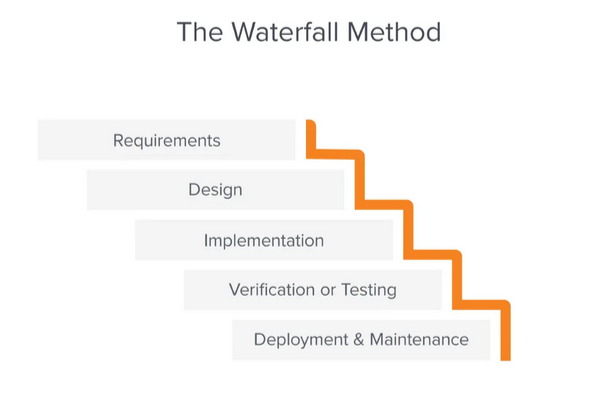
\includegraphics[width=0.8\textwidth]{Implementation/Methodology/Waterfall.png}
    \caption{An overview of a Waterfall workflow \autocite{adobeWaterfallMethodologyProject}. \label{fig:Waterfall}}
\end{figure}

\noindent Waterfall begins by ascertaining all project requirements for all stages of the project, which 
would include costs, risks, associated dependencies and overall timelines for completions of each stage.
Following this is the design stage, where a general high-level design is created to demonstrate the 
project, and this design is then acted upon and implemented in the implementation stage. Then, the 
implementation is rigorously tested before its eventual deployment.

\para It is a methodology with a strong reputation due to its clear structure, with all necessary facts and figures 
being calculated in the requirements stage before any designs or development occur. The clear structure allows 
progress to be easily measured against each predefined milestone.

\para Though, despite these advantages, Waterfall brings with it some clear disadvantages - the first of which 
being that with all requirements being defined at the very beginning of the project's development,
it introduces significant difficulty should there be any further requirements specified during development. This would also 
bring in the second disadvantage known as 'deadline creep' \autocite{adobeWaterfallMethodologyProject}; 
if one stage is delayed, such as by request for additional features, this would then impact all subsequent stages. 

\subsection{Agile}
The second methodology considered was another highly reputed software development methodology known as Agile.
Unlike Waterfall which defines all stages and requirements at the beginning, Agile is a highly iterative methodology with steps
known as 'sprints' which are frequently repeated, providing a more incremental approach to development. Each of these sprints
would represent a small part of the program, eventually building up to the full version.

\para As depicted in Figure \ref{fig:ExampleAgileSprint}, 
Agile sprints begin by planning the overall aims of that particular sprint. Similarly to Waterfall, a high-level
design is then created and developed, before being rigorously tested. This is also one of Agile's key benefits; the 
constant testing of the small parts developed in each sprint helps ensure that all bugs can be rectified, unlike 
Waterfall where the whole product is tested and some smaller elements with bugs could potentially be overlooked.
After testing, the product of that sprint is deployed and reviewed. Then, the cycle begins anew with another 
sprint.

\begin{figure}[H]
    \centering
    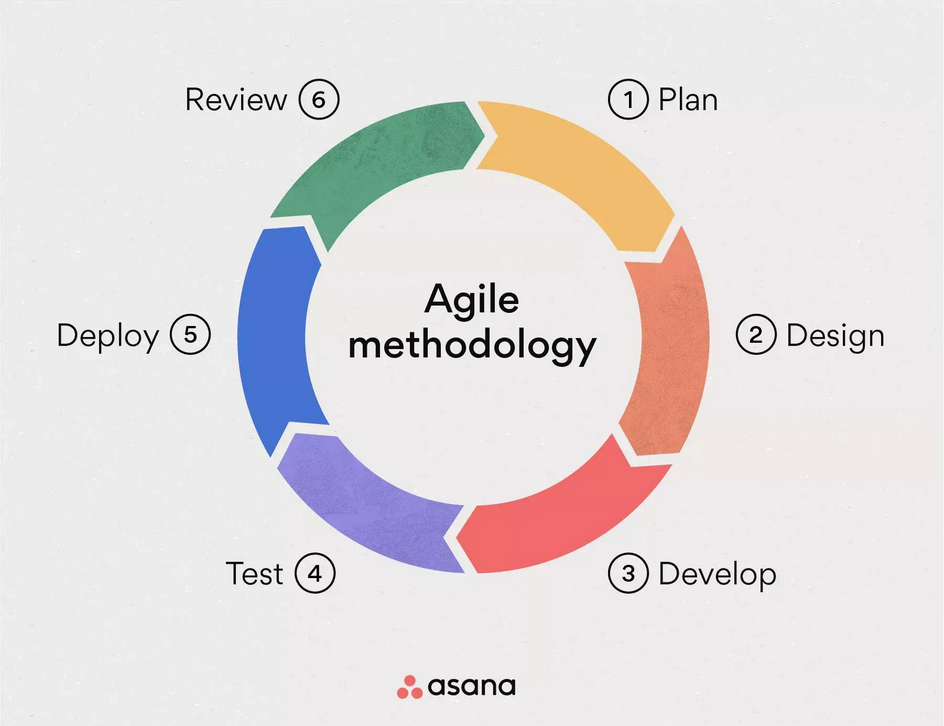
\includegraphics[width=0.65\textwidth]{Implementation/Methodology/Agile.png}
    \caption{An overview of an Agile sprint \autocite{asanaWhatAgileMethodology}\label{fig:ExampleAgileSprint}}
\end{figure}


\noindent The most prominent key benefit of Agile is its sprint-based iterative nature that allows for requirements to shift 
throughout development without major disruption. Furthermore, this incremental process minimises the risk of total project 
failure as usable components are constantly produced. In business environments, Agile also allows for enhanced teamwork, though 
this will not be present in this particular project.

\para As with Waterfall, Agile is not without drawbacks. Agile's most notable drawback is known as 'scope creep' \autocite{malsamWhatScopeCreep2024},
which occurs when requirements are continually added to a point where development can never truly end; the product continues to expand 
far beyond its original intentions to the point where maintenance becomes extremely difficult or outright impossible with an 
ever-expanding codebase. Furthermore, it is possible that because of this, the end product can be almost entirely different to its original concept.

\subsection{Comparison and decision}

Both methodologies bear strong benefits and drawbacks. The particular choice for this project is Agile, primarily because of the reduced 
risk through constant testing and also for its deeply flexible nature allowing the requirements of the project to potentially shift 
over time as needed, unlike Waterfall where this could cause major deadline creep. Additionally, the time-sensitive nature of this project 
best suits Agile's fast incremental sprints rather than the slower, more methodical Waterfall.

\section{Potential limitations and mitigations}\label{sec:Limitations}
The project as a whole bears some limitations of its own that may hinder the development process or the final product.

\subsection{Time}
The project is likely to take a considerable amount of time to develop to the excellent standard desired. This poses an issue 
in balancing time throughout the academic year alongside four other modules each with their own independent deadlines and workloads
of similar scale. As such, it is possible that if the product has issues, they could have been remedied with additional development 
time.

\para To mitigate this risk, a Gantt chart was developed to model the overall project timeline, and can be found in Appendix A.
% !!!!!!!!!!!!!!!! GANTT
% ! Didn't the proposal have risk assessments?

\subsection{Cost}
Due to the inability to use OpenAI's LLMs on a local device because of both their proprietary nature and extreme hardware requirements,
their public API will need to be used instead. This incurs a financial cost for every query sent and response received from the LLM,
dependent on the model chosen. For example, GPT-4o has a cost of \$2.50 per 1,000,000 input tokens \autocite{openaiPricingOpenAIAPI}.
Throughout the development and testing processes in each sprint, a cost will slowly begin to accrue.

\para Mitigating risks posed by potential cost constraints will be remedied by identifying the optimal model, which was decided to 
be gpt-4o-mini. The project has a limited budget due to it being a solo endeavour, though using a somewhat less intelligent model 
will greatly mitigate the risk of overspending while only compromising slightly on answer quality. 

\subsection{Experience}
Personally, I have never worked with LLM APIs before, nor the frameworks used to create apps with them such as LangChain. As such,
it is highly likely that many issues will be faced during the development process as I am forced to learn a tech stack that is completely 
new to me. This also links back to the previously mentioned time constraint, with the time taken to learn the modules used being time that 
could have been spent on development had I known them ahead of time.

\para To address this risk, time will be budgeted to allow for thorough research into the necessary tech stack to ensure that the project 
can be completed to a suitable standard.

\subsection{Independence}
This project is a solo venture with no support from others. As such, the previously mentioned issues of time and cost are entirely 
my own burden and responsibility. 
% ! Can anything really be said here other than 'I just dealt with it'?

\subsection{LLM Unpredictability}
LLMs are an extremely useful tool, being able to execute instructions given to them in natural language. However, without specific tuning, 
an LLM will not give the same response to the same prompt every time it is given. While this does add a sense of personality which could 
aid with a chatbot, it may risk answering questions incorrectly. This also can make LLM-based programs extremely challenging to debug due 
to this lack of reproducibility.

\para In an effort to mitigate any potential risk of LLM unpredictability, the chatbot's 'temperature' parameter will be set to 0, 
which will make its responses more static. This means that the chatbot should provide the same answer any time it is asked a certain 
question unless there are external circumstances (previous conversation history, etc.). 

\subsection{LangChain Documentation}
LangChain will be a critical element in this project's development, serving as the backend framework that the chatbot will run on.
Therefore, it is mandatory that I learn about it in order to produce a functional product, which would typically involve reading the 
documentation as is common when learning new modules. However, LangChain's documentation is frequently outdated and/or references 
functions or classes that have since been deprecated, without the documentation being updated. LangChain also frequently deprecates classes 
and functions with each new update, meaning that finding the current optimal methods for specific aims can be challenging.

\para Despite this risk, LangChain is recognised as a good framework for developing LLM-based applications and there are other 
resources that can be learned from that are not the documentation page, such as tutorial videos and blogs. Through using alternative 
resources alongside the official documentation, it should be possible to use LangChain to a good standard to produce an end product 
of suitable quality.

\section{Design}
Before any design concepts can be created, it is first necessary to establish what is being designed. Therefore, the functional and 
non-functional requirements for the chatbot were considered.

\subsection{Requirements}\label{sec:Requirements}
\subsubsection{Functional Requirements}
The following requirements are deemed essential to the chatbot's function, and the project cannot be considered complete unless they 
are fulfilled:

\begin{itemize}
    \item The chatbot must interpret and respond to answers in English.
    \item The chatbot must accept text queries.
    \item The chatbot must respond using text.
    \item The chatbot must be accessible at all times.
    \item The chatbot must supply BCU-related information.
    \item The chatbot must answer at least 75\% of BCU-related queries correctly.
    \item The chatbot must have a GUI for ease of use and accessibility.
    \item Multiple users must be able to use the chatbot at the same time.
\end{itemize}

\subsubsection{Non-functional Requirements}
The following requirements, while not essential, would be beneficial if fulfilled:

\begin{itemize}
    \item The chatbot should respond to queries within 10 seconds.
    \item The chatbot could allow for voice input and output.
    \item The chatbot could be deployed on an existing messaging service such as Teams.
\end{itemize}

\subsection{Concept diagrams}

Figure \ref{fig:ConceptDiagram} depicts a theoretical interaction with the chatbot from the frontend user's perspective created 
early in development.

\begin{figure}[H]
    \centering
    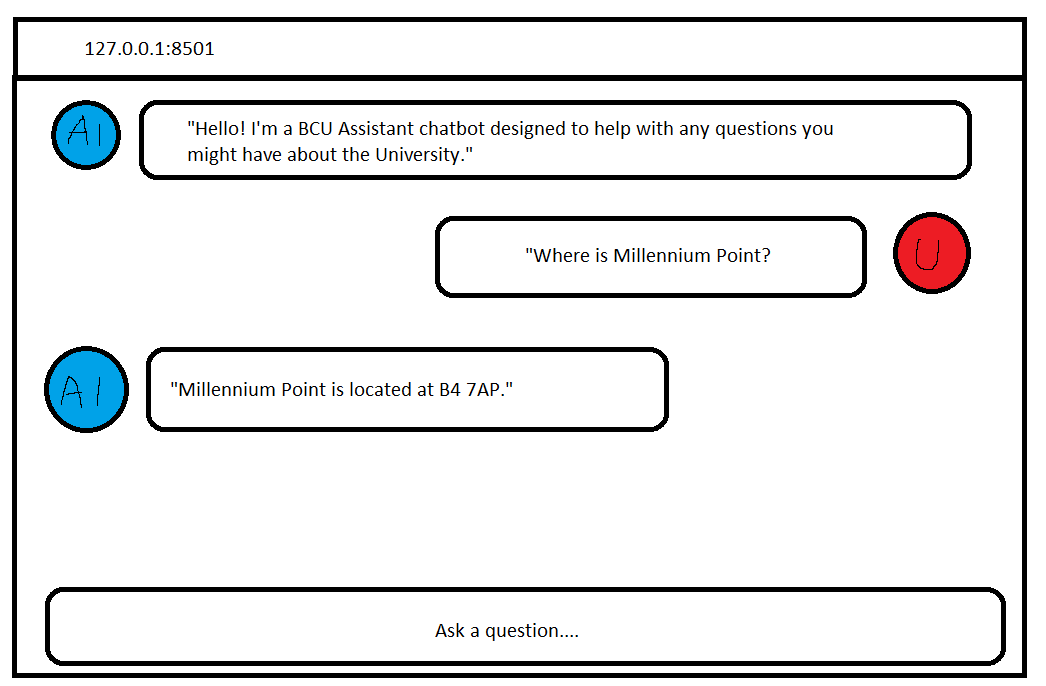
\includegraphics[width=\textwidth]{Implementation/ConceptDiagram.png}
    \caption{An early visualisation of a conversation.\label{fig:ConceptDiagram}}
\end{figure}

\noindent Users will have a clearly labelled text input box, and a messaging interface similar to other text messaging apps 
which they would hopefully be familiar with allowing for them to quickly understand how to interact with the chatbot.
This version of the chatbot would be hosted locally, though with additional time and resources it could instead be hosted on a 
dedicated domain or as part of another service.

\para Figures \ref{fig:EmbedFlowchart} and \ref{fig:RAGFlowchart} depict how the backend of the chatbot should work, including the 
storage of BCU data and how the chatbot will query it.

\begin{figure}[H]
    \centering
    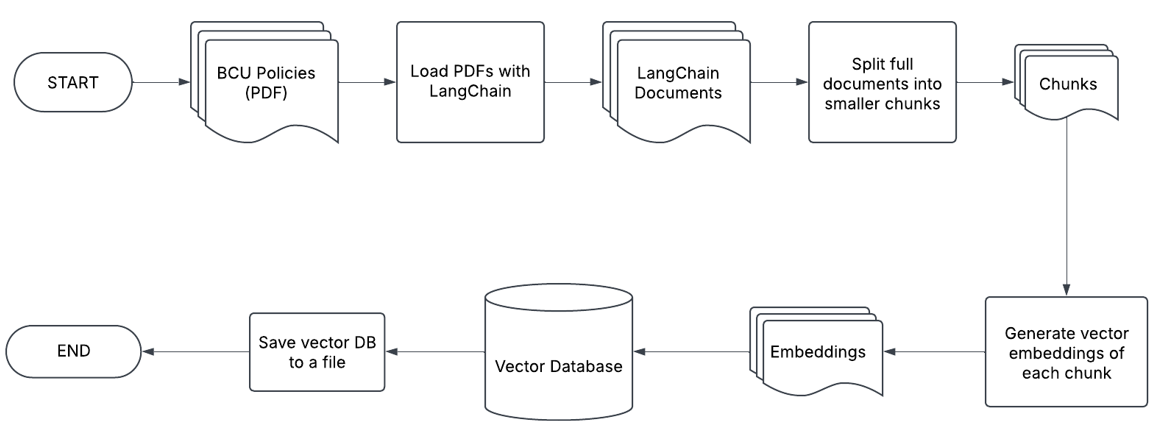
\includegraphics[width=\textwidth]{Implementation/LucidEmbedFlow.png}
    \caption{The flowchart for the PDF embedding procedure.\label{fig:EmbedFlowchart}}
\end{figure}

\noindent BCU's policies are publically available on their website \autocite{bcuPoliciesProcedures}, with policies valid during the 2024/25 academic
year being used in this project. The planned use case for these policies was to download them locally and then process them using LangChain as a 
wrapper to split the PDFs into smaller chunks and embed them into a vector database. LangChain provides classes for direct PDF loading and 
conversion into its own "Document" format, and also provides functions to vectorise each chunk using any embedding model, with OpenAI's 
text-embedding-3-small being used. 

\para After the embedded chunks are stored, the database generated from this process is stored locally. This means that the chatbot will operate 
both locally and on the cloud, with vector similarity searches being executed on the chatbot host device and the proprietary gpt-4o-mini LLM running 
on an OpenAI server.

\begin{figure}[H]
    \centering
    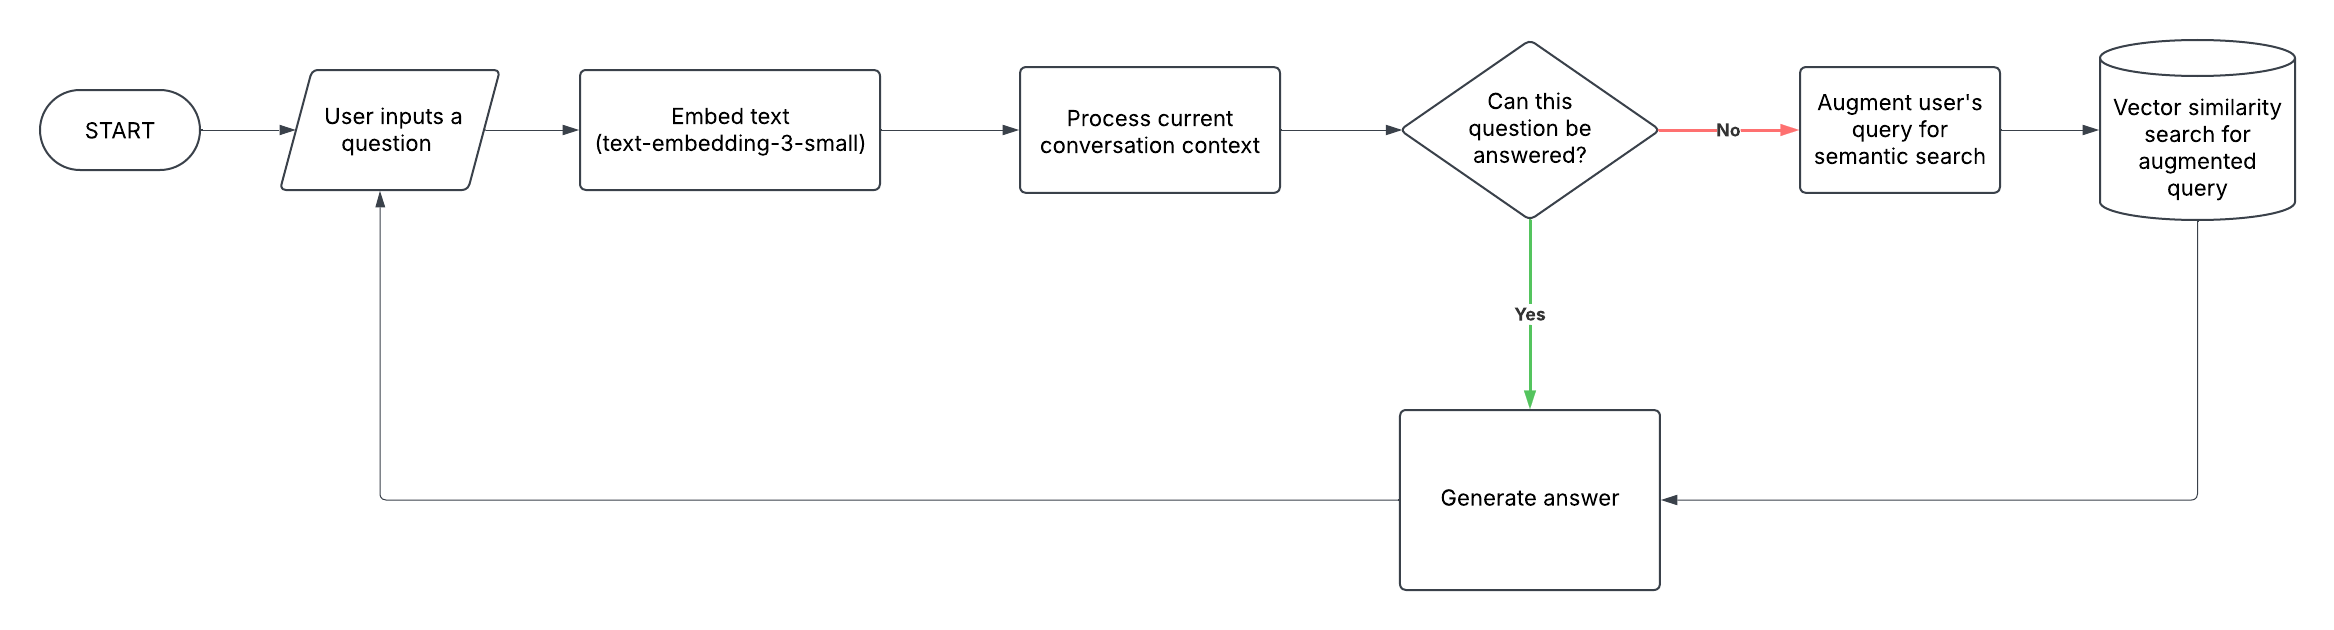
\includegraphics[width=\textwidth]{Implementation/LucidRAGFlow.png}
    \caption{The flowchart for the answer generation procedure.\label{fig:RAGFlowchart}}
\end{figure}

\noindent Users will input prompts as natural language to the chatbot, which will then vectorise them using the same embedding model used 
to embed the BCU policies. This is a necessary procedure as different embedding models will yield different outputs, meaning that if the same 
model was not used for the storage of policies and conversion of user queries, answers would be completely incorrect. 

\para In the interest of saving costs and reducing response times, the chatbot will ideally not query its university information vector store 
unless it cannot answer a question without it. This is because appending the university information, even in small amounts, would 
greatly increase the token usage of each individual prompt. To do so, the chatbot will review the existing conversation when it receives a 
prompt. If it already has the answer to the user's question in previously retrieved context, there will be no need to perform another search 
and duplicate pre-existing context.

\para Another way that the chatbot may choose not to query the database is if the user's prompt can already be answered by the LLM. This may 
occur with very simple queries, such as "Hello!" or "My name is Lewis." In either of these example scenarios, the chatbot should not query the 
database, as the LLM should be capable of responding to generic greetings and remembering a user's name. Additionally, answers that do not 
require similarity searches should be answered considerably quicker, and would make the user experience feel much smoother if they are not 
having to wait a long time between responses as previously detailed in Section \ref{sec:Requirements}. 

\para This decision functionality would be provided by LangGraph, and is detailed 
further in Section \ref{sec:ChatbotBackend}.




    \section{Implementation}\label{sec:Implementation}
% ! Nuclear option: Linux dual-boot and screenshot as you go on it.

\subsection{Software requirements}
% Talk about Visual Studio Code.
% Talk about Python and the modules themselves. Did any of them have logins?
% Talk about OpenAI setup.
The project was developed using Visual Studio Code as a development environment and Python as the programming language.
Both of these are available freely with no limitation for academic use.

\para Many Python modules were used, with the UV package manager \autocite{astralUv} being used for their installation 
due to its own high speed and ease of use. The version of Python used was 3.10.16 to ensure compatibility with the wide variety 
of modules used, which are detailed in Table \ref{tab:PythonModules}.

\begin{longtable}{ | p{0.25\textwidth} | p{0.7\textwidth} | }
    \hline
    \cellcolor{blue!25} Module(s) & \cellcolor{blue!25} Purpose \\
    \hline
    langchain & The framework used to handle LLM interactions, as well as embedding documents and user queries. \\
    \hline
    langchain-community & Provides additional helper classes and functions to assist development. \\
    \hline 
    langchain-openai \newline 
    openai & Provides the functions used to interact with OpenAI models such as gpt-4o-mini and text-embedding-3-small in LangChain. \\
    \hline 
    langgraph & Used to create a directed sequence of events for the chatbot to execute. A major part of the backend, further described 
    in Section \ref{sec:ChatbotBackend}. \\
    \hline
    pdfminer-six \newline 
    pypdf & Dependencies of LangChain for PDF reading. \\
    \hline 
    Streamlit & Used as the frontend of the chatbot and also stores the conversation in memory. Described further in Section 
    \ref{sec:ChatbotFrontend}. \\
    \hline
    \caption{The Python modules used in the project's development.}\label{tab:PythonModules}
\end{longtable}



\subsection{Data storage}
% Talk about getting University policies from their site. Provide URL or Harvard reference it?
% Talk about your own added info document you made in LaTeX.
% Talk about embedding the policies.
The backbone of this project is the BCU-related data that the chatbot will pull from when queried.
The vast majority of this data was sourced from the official Birmingham City University website \autocite{bcuPoliciesProcedures},
where individual policies are stored as PDF files for public download without any access limitations or restrictions.
An observation made through an analysis of many of the policies was that none of them explicitly state key information about the university,
such as campus building locations or information about its student union. Therefore, an additional document of my own creation with \LaTeX
was included amongst the downloaded data. This document contained key information about BCU itself, with information on campus addresses 
and miscellaneous helpful information for students.

\para With all documents downloaded or created, the next stage would be to incorporate them in a format an LLM can interpret. This introduces 
LangChain, a popular framework for LLM app development \autocite{langchain_introduction_nodate}, which provides helper classes to directly read 
PDF files from a directory and split the text data within into smaller chunks, as seen in Figure \ref{fig:LangChainDocumentLoader}.

\begin{figure}[H]
    \centering
    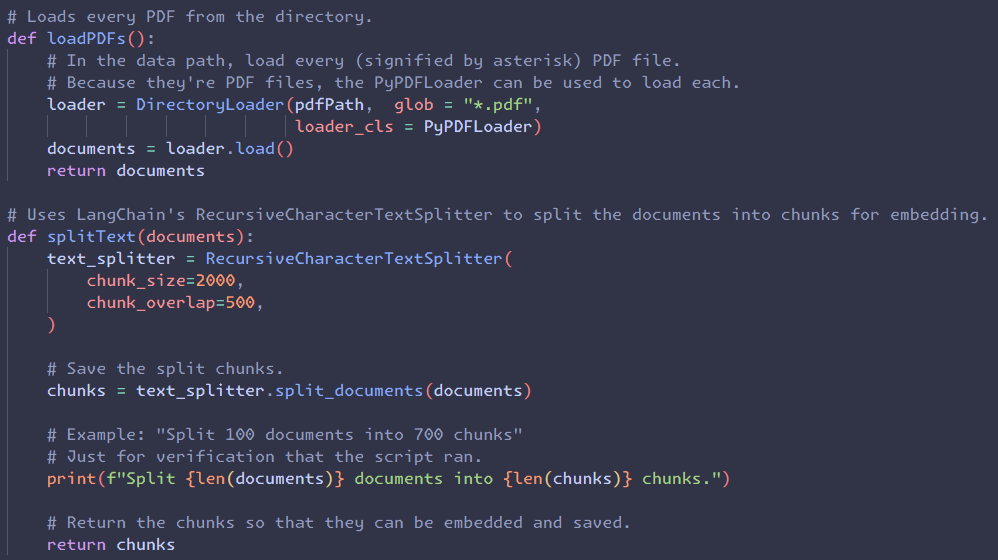
\includegraphics[width=0.8\textwidth]{Artefact/DocumentLoader.png}
    \caption{Code used to load all PDFs from the Policies directory and split them into chunks. \label{fig:LangChainDocumentLoader}}
\end{figure}

\noindent Multiple chunk sizes and overlaps were tested during the artefact's development, with an eventual settlement on 2000 character 
chunks with 500 character overlaps being used. Maximising the size of chunks is a key part in assisting the chatbot's retrieval process,
as it will be able to fetch more data with a single query which allows it to answer questions with greater detail and factual accuracy.
The chunk overlap defines how many characters appear across multiple sequential chunks, ensuring that key information is unlikely to be 
split over multiple chunks where the chatbot then may be unable to cite it. LangChain's RecursiveCharacterTextSplitter also provides 
additional arguments for a custom length function if desired, though there was no need in this project, as well as adding start indexes 
to each vector, which adds metadata stating the numerical ID of each chunk as determined by the sequential order they are split in. 

\para Once these chunks have been created, they must then be embedded as vectors, which will allow an LLM to interpret them. These 
vectors were then stored in a Facebook AI Similarity Search (FAISS) database as researched in Section \ref{sec:LitReviewRAG}, which 
ensured that the policies only needed to be embedded once rather than every time the chatbot was run, and would be retrieved 
at high speeds thanks to FAISS' efficiency.

\begin{figure}[H]
    \centering
    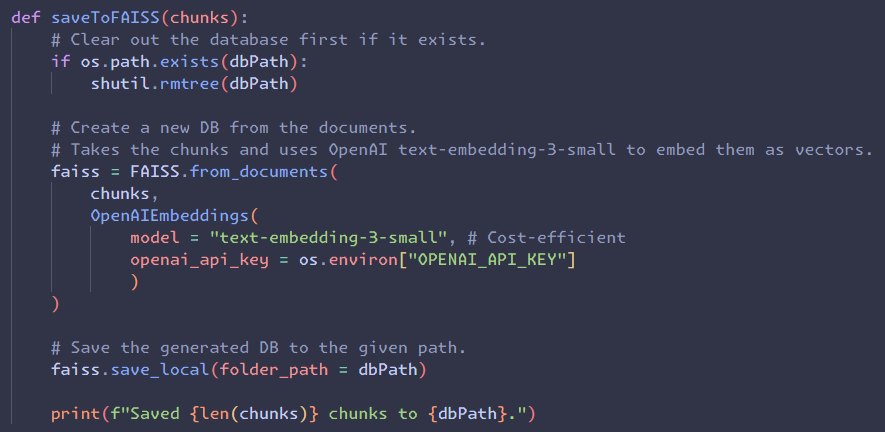
\includegraphics[width=0.8\textwidth]{Artefact/SaveToFAISS.png}
    \caption{Code used to embed and store the chunks into a FAISS DB. \label{fig:LangChainStoreFAISS}}
\end{figure}

\noindent Firstly, any existing database in the specified directory is cleared to ensure that there are no I/O errors when attempting 
to save to the directory. LangChain provides wrapper functions for both the embedding and storage of this data, making it a smooth 
and simple process in very few lines of code. 

\para The embedding model used is OpenAI's text-embedding-3-small model \autocite{openai_vector_nodate}. The motivation behind the use of this model 
was primarily due to its cost efficiency, with OpenAI approximating 62,500 pages can be embedded for each dollar spent. For each 
2000-character chunk, the embedding model translates it into vector space for the LLM's interpretation. The vectors are produced based on the 
semantic similarities of each word as previously discussed and visualised in Section \ref{sec:LitReviewNLP}. 

% ! Screenshot of this running if possible.



\subsection{Backend code}\label{sec:ChatbotBackend}
% Talk about LangChain and LangGraph.
As previously mentioned, the core functionality of the chatbot was developed using the LangChain and LangGraph frameworks. LangChain in particular
simplifies the development process by providing various functions and classes for quick and easy integration with necessary services such 
as FAISS and the OpenAI API, with LangGraph defining the chatbot's structure as depicted in Figure \ref{fig:ChatbotLangGraph}. 

\begin{figure}[H]
    \centering
    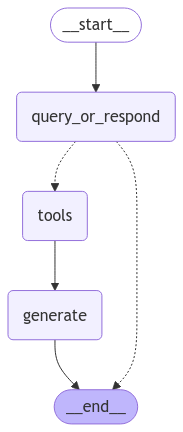
\includegraphics[width=0.3\textwidth]{Artefact/LangGraph.png}
    \caption{The graph for the chatbot. \label{fig:ChatbotLangGraph}}
\end{figure}


\para Before detailing each node of the graph, it is first necessary to establish some prerequisite variables such as the LLM itself. 
The LLM used is OpenAI's gpt-4o-mini due to cost-efficiency. The difference in performance between 4o-mini and 4o was deemed not significant 
enough for the price increase of 1500\% per 1 million tokens in relation to 4o-mini \autocite{openaiPricing}, especially considering that 4o-mini
performs suitably for the task at hand.

\para Figure \ref{fig:PrelimVariables} shows each of the variables being established, including the LLM, 
via LangChain's 'init\_chat\_model' function. The LLM is initialised with a temperature of 0, which means that it should give the same 
answer to the same prompt whenever it is given. As mentioned, this does reduce the 'personality' of the chatbot, though it greatly helps 
to reduce the potential for hallucinations in a Q\&A RAG scenario such as this one.

\begin{figure}[H]
    \centering
    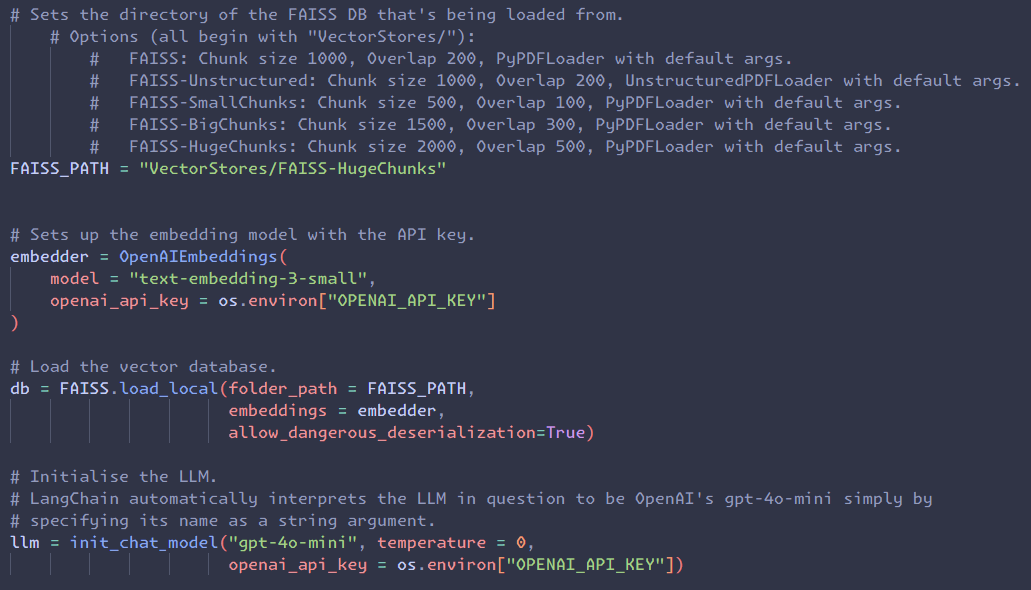
\includegraphics[width=\textwidth]{Artefact/PrelimVariables.png}
    \caption{Establishing prerequisite variables for the chatbot. \label{fig:PrelimVariables}}
\end{figure}

\noindent Thorough experimentation with the chunk sizes previously discussed in Figure \ref{fig:LangChainDocumentLoader} occurred during 
development, with the eventual decision of settling on the 2000-character chunks being made due to its more reliable performance on a set 
of sample questions discussed in Chapter \ref{ch:Evaluation}. Following the relative directory of the FAISS database being set, the 
% ! Change "chapter" to the specific relevant section when it's written.
OpenAI embedding model is once again used so that similarity searches may be performed on the database. An additional argument,
'allow\_dangerous\_deserialization', is given when loading the database. When a FAISS database is saved using LangChain, it is saved as a 
serialized file known as a Pickle file, using a .pkl file extension. It is possible for malicious code to be embedded inside these files
which could be executed when they are deserialized. However, as the files were generated specifically for this project and their contents 
are already known, it is safe to deserialize them.

\para With the prerequisite variables established, the first node of the graph was created. This is the core functionality of the LangGraph 
module, which builds on LangChain by defining an app's workflow 
as nodes and edges on a graph \autocite{langgraphLangGraph}. In development, these nodes and edges can be created, with support for conditional 
edges that ensure certain nodes such as tool calls only activate when necessary. This allows for the creation of self-directed agents which make 
decisions independently, with this functionality being used in the chatbot to decide whether a response needs BCU-related context or not. This 
occurs in the first node and entry point of the graph: the 'query\_or\_respond' node.

\begin{figure}[H]
    \centering
    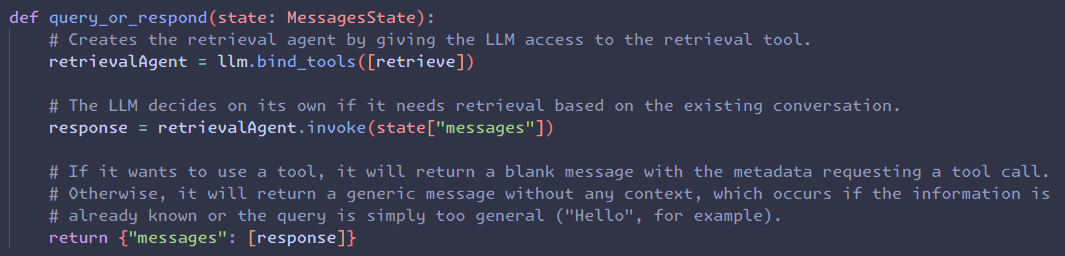
\includegraphics[width=\textwidth]{Artefact/QueryOrRespond.png}
    \caption{Code used for the 'query\_or\_respond' graph node. \label{fig:QueryOrRespond}}
\end{figure}

\noindent This function clearly demonstrates LangChain's abstractions of the backend functionality; these three lines of code
serve as the entire decision-making logic for this node, as the LLM itself will decide whether it can immediately answer the user's query,
such as in a scenario where the information they are requesting is already known from earlier in the conversation, or if their query is too 
general such as stating their name. If the LLM decides it cannot answer the query with the information it currently has available within 
the conversation, it will instead invoke the left conditional branch of the graph in Figure \ref{fig:ChatbotLangGraph} by calling on the 
retriever tool denoted in Figure \ref{fig:RetrieverTool}.

\begin{figure}[H]
    \centering
    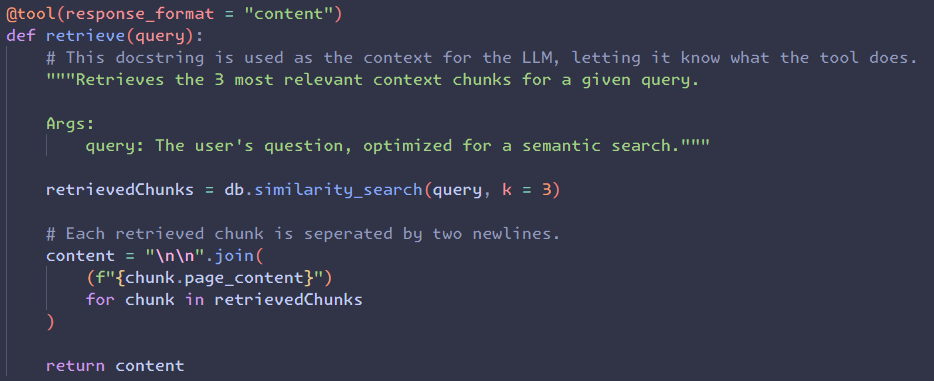
\includegraphics[width=\textwidth]{Artefact/Retriever.png}
    \caption{Code used for the retrieval tool. \label{fig:RetrieverTool}}
\end{figure}

\noindent Using the '@tool' decorator informs LangChain that the following function is a tool to be used by the LLM.
% The tool's response format is set to content, meaning that it will return the results as a LangChain 'ToolMessage', 
% which is beneficial for the frontend as these can be manually hidden from the user. 
The retriever tool itself is simplistic 
in function: it will perform a semantic search on the FAISS database based on the user's query. LangChain enforces that all 
tools require a Python docstring explaining their function, as the LLM will read this docstring to understand what the tool 
is and how to use it. By specifying that the 'query' argument should be optimised for a semantic search, the 'query\_or\_respond'
node will output a modified version of the user's query as the input to the tool, which is further discussed in Section 
\ref{sec:ChatbotFrontend}. 
% ! Show this happening? 

\para When the 3 most similar chunks have been retrieved as defined by 'k' in the similarity search method, the text of each chunk 
is saved and separated by two newline characters to assist the LLM in understanding they are not part of the same text. The large 
text block is then returned as this tool's output, ready to then be passed into the 'generate' node. 

\begin{figure}[H]
    \centering
    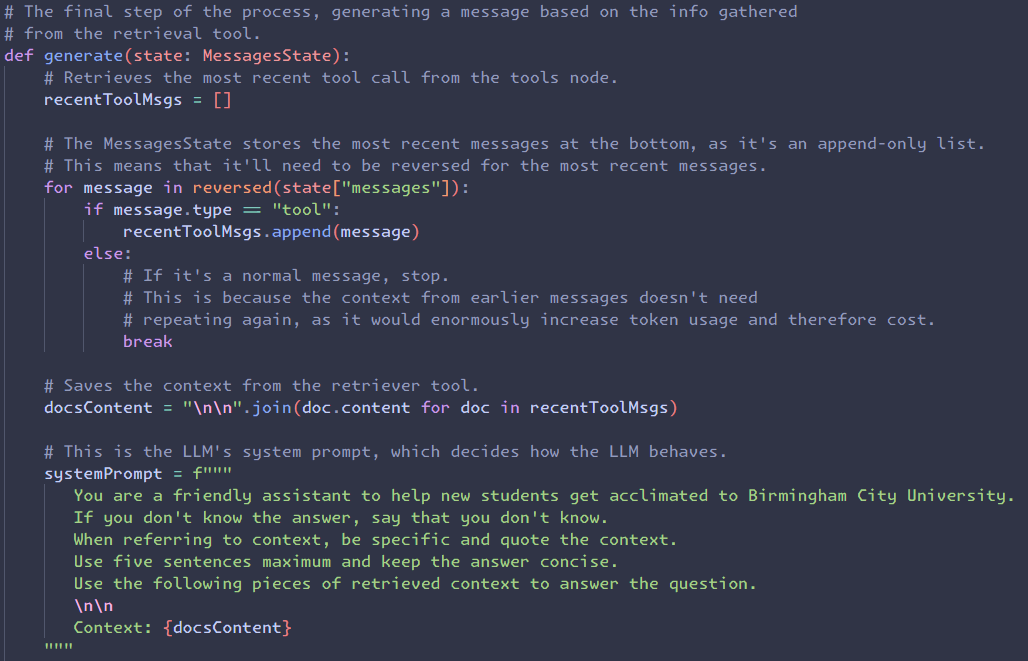
\includegraphics[width=\textwidth]{Artefact/Generate1.png}
    \caption{Code used for the 'generate' node (1/2). \label{fig:Generate1}}
\end{figure}

\noindent The 'generate' function is the largest function of the chatbot, and is split across 
Figures \ref{fig:Generate1} and \ref{fig:Generate2}. In the interests of saving 
cost, time and the potential risk of maximising the LLM's context window, the most recent retrieval tool 
call is saved. This tool call contains the RAG context from the retrieval tool, and will be at least 
6,000 characters in length due to the previously mentioned chunk sizes and amount of chunks retrieved.
This most recent tool call is the only context given to the LLM to reduce the token cost of each prompt 
and to mitigate any potential confusion if the LLM is given thousands of words of input context.

\para The retrieval tool returns three LangChain Document objects, each containing one chunk.  
Therefore, the content of each of these Documents is extracted and saved before being appended to the 
LLM's system prompt.

\para The system prompt is a massive part of LLM usage, and almost entirely dictates what the LLM will do 
based on any given input. The prompt is written in natural language which is interpreted by the LLM as a set 
of instructions to follow at all times. As such, the prompt given for the chatbot defines that it is 
a BCU assistant which should specifically quote context and keep all answers brief (for cost efficiency).
This prompt was found to be highly effective, with the LLM responding with mostly satisfactory results as 
detailed in Chapter \ref{ch:Evaluation}.

\begin{figure}[H]
    \centering
    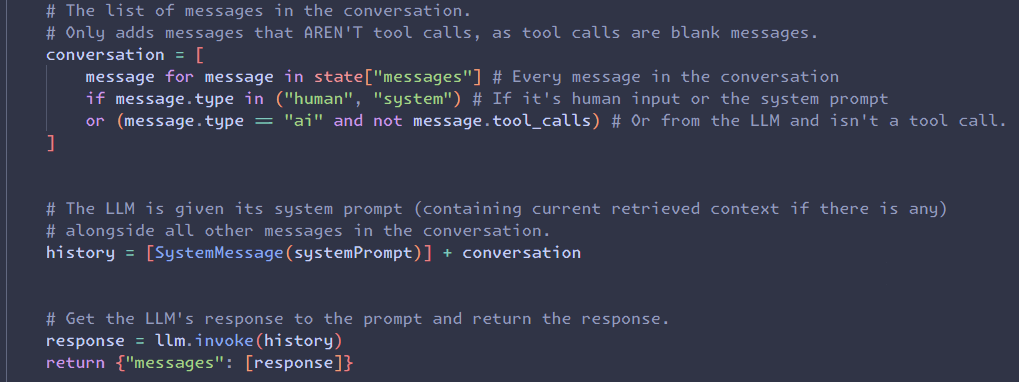
\includegraphics[width=\textwidth]{Artefact/Generate2.png}
    \caption{Code used for the 'generate' node (2/2). \label{fig:Generate2}}
\end{figure}

\noindent With the system prompt prepared, the LLM should also account for the current conversational 
history, which is retrieved from the LangGraph MessagesState. The MessagesState is an append-only list 
containing all messages in the current conversation, stored as a HumanMessage, AIMessage, or SystemMessage.
These are three LangChain objects used to represent the various actors in a conversation: the human user,
the LLM and the system prompt.

\para When retrieving the current conversation, tool calls are excluded. This is because through experimentation,
it was discovered that when the chatbot calls on a tool, it generates a blank message with metadata indicating a
tool call. This blank message is not relevant, and therefore does not need to be included in the conversational history.
% This is because the context from 
% tool calls is written into the system prompt as seen previously in \ref{fig:Generate1}, and also saving 
% these messages would cause all context to be duplicated, doubling token costs. 
% ? One or the other.

\para Finally, the new system prompt is inserted as the most recent message in the conversation, and the LLM
is invoked with the filtered conversation history, with the generated response being returned.

\begin{figure}[H]
    \centering
    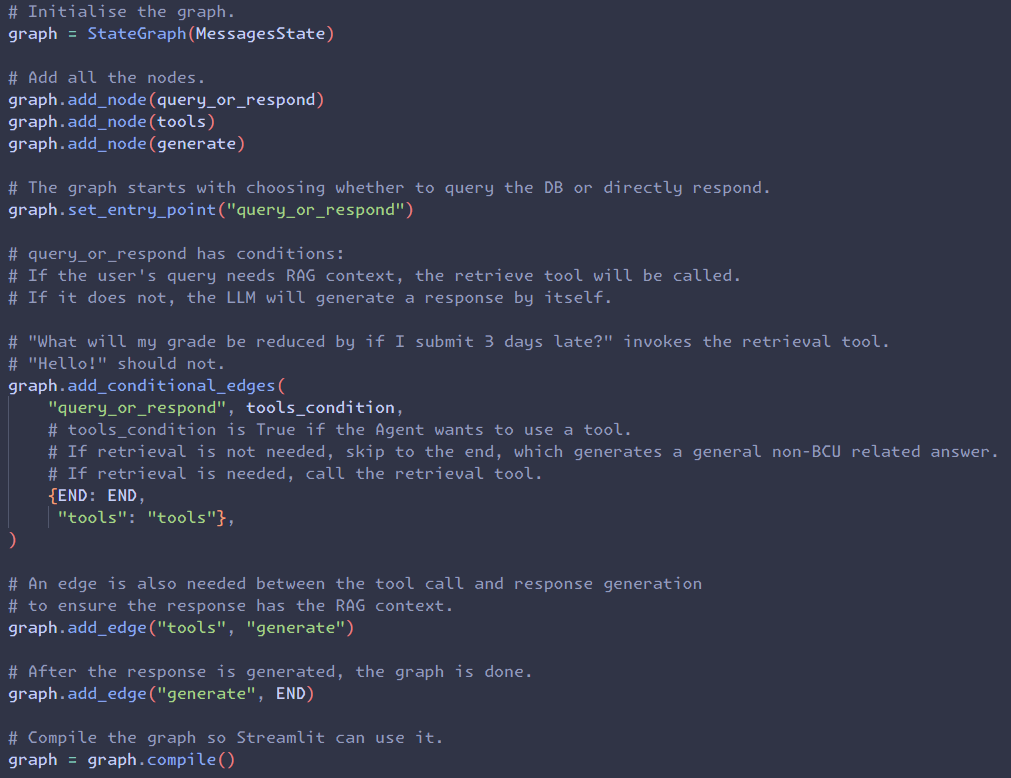
\includegraphics[width=\textwidth]{Artefact/LangGraphCode.png}
    \caption{Code used to form the graph. \label{fig:LangGraphCode}}
\end{figure}

\para To conclude the chatbot's backend Python script, the LangGraph is created using the conditions mentioned 
previously. A particularly helpful feature of LangGraph for this scenario was 'tools\_condition', which is
set to True if the LLM calls on a tool, and False if it does not. Based on this condition, the graph will either 
go down the left branch, invoking the retrieval tool and generating a contextualised response, or it will skip 
directly to the end, where the LLM will generate a generic answer without any RAG.


\newpage 

\subsection{Frontend code}\label{sec:ChatbotFrontend}
% Talk about Streamlit.
% Show example conversations here or perhaps make another section for them.
The chatbot's frontend GUI was created using the Streamlit package, which allows for the creation of visually appealing, dynamic and 
responsive web apps through simple Python code \autocite{streamlitStreamlitFasterWay2021}. Figure \ref{fig:StreamlitInitPage} shows 
the initial variables set for the page's structure.

\begin{figure}[H]
    \centering
    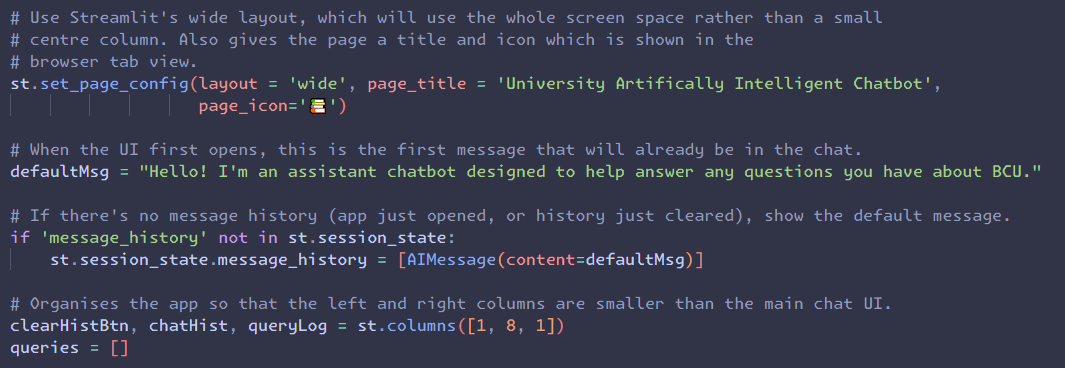
\includegraphics[width=\textwidth]{Artefact/Streamlit/Backend/PageInit.png}
    \caption{The variables defining the frontend page's structure. \label{fig:StreamlitInitPage}}
\end{figure}

\noindent Streamlit provides many helpful methods and variables for creating the frontend GUI, allowing for the page layout to be 
quickly defined using 'set\_page\_config', where the wide layout was used to ensure the app fills the screen, and the title and an icon 
for the browser tab are also provided. 

\para When the app initially opens, it would by default open to a mostly blank page. To remedy this, a default message was provided 
explaining what the chatbot is, which will always show as the first message in the conversation. This is performed by validating that 
the current session's message history is empty before inserting the default message.

\para Following this, three columns are set up on the page: a small column containing a button to clear the current message history,
a large column containing the main chat UI, and another small column showcasing the queries being given to the FAISS database by the 
chatbot, which would be none at the time of startup, so an empty list is defined.

\para After the page's structure is defined, the functionality of each of the three columns is established as depicted in Figures \ref{fig:StreamlitLRColumns}, \ref{fig:StreamlitMainColumn1} and \ref{fig:StreamlitMainColumn2}.

\begin{figure}[H]
    \centering
    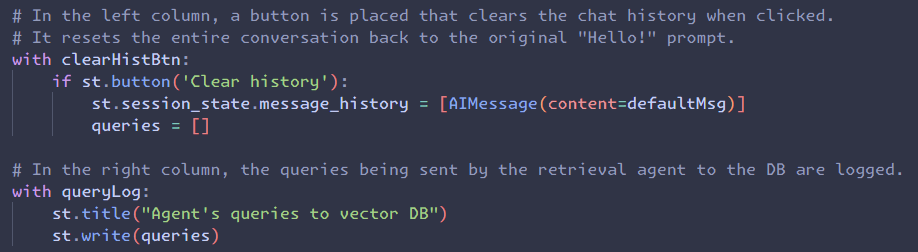
\includegraphics[width=\textwidth]{Artefact/Streamlit/Backend/LRColumns.png}
    \caption{Defining the left and right column functions. \label{fig:StreamlitLRColumns}}
\end{figure}

\noindent The left column ('clearHistBtn') has a button placed in it which will clear the current conversational history when clicked,
and also empty the list of queries to the database. This button effectively resets the app to its initial opening state.

\para The right column ('queryLog') outputs all the agent's queries which it has given to the vector database. The queries themselves are 
retrieved within the main column of the app, 'chatHist'.

\begin{figure}[H]
    \centering
    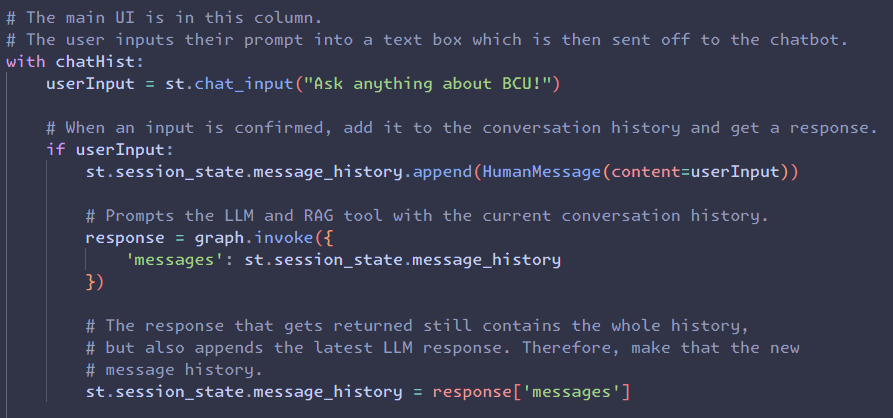
\includegraphics[width=\textwidth]{Artefact/Streamlit/Backend/MainColumn1.png}
    \caption{Defining the main column function (1/2). \label{fig:StreamlitMainColumn1}}
\end{figure}

\noindent The user's input box is established, and when an input is given, it is added to Streamlit's active 
conversation history, which is then used to invoke the chatbot's LangGraph. When the chatbot responds, it returns 
the entire conversation history once again, this time containing the chatbot's latest response. Therefore, this is used 
to overwrite the existing Streamlit history.

\para With the core prompting functionality set, the Streamlit UI for this column then needed to be established as depicted 
in Figure \ref{fig:StreamlitMainColumn2}.

\begin{figure}[H]
    \centering
    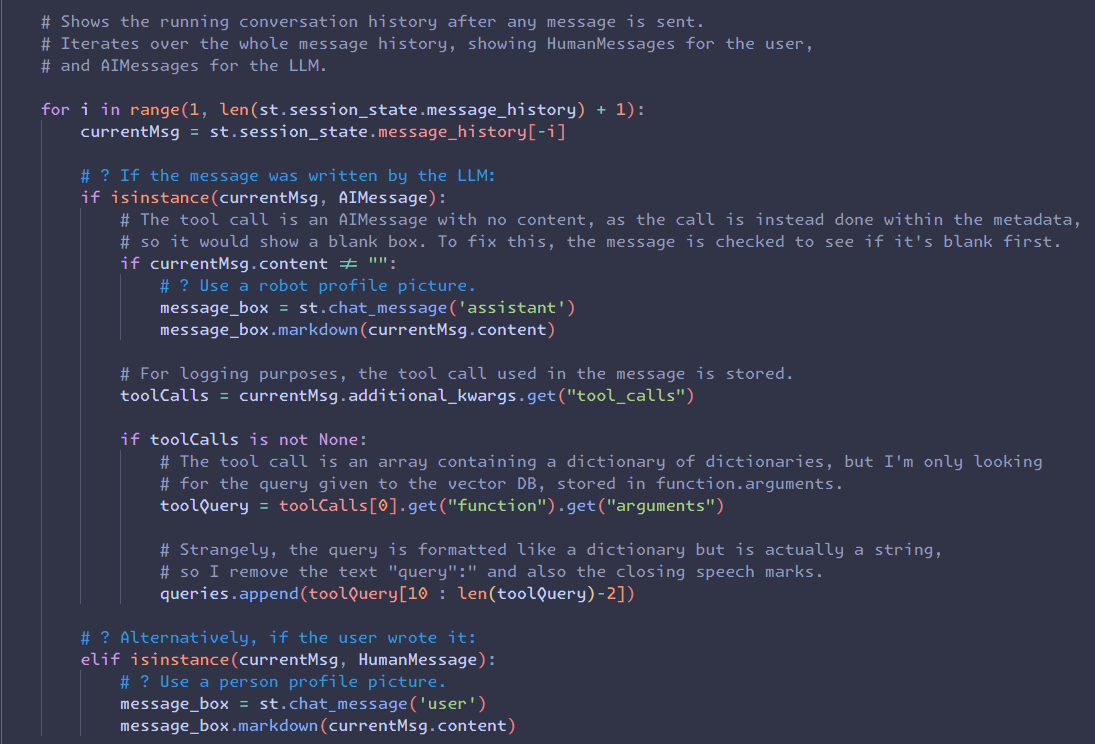
\includegraphics[width=\textwidth]{Artefact/Streamlit/Backend/MainColumn2.png}
    \caption{Defining the main column function (2/2). \label{fig:StreamlitMainColumn2}}
\end{figure}

\noindent By iterating over each message in the conversation, logic is established to determine whether the message should 
use a human profile picture or a robot profile picture, representing the user and chatbot respectively. Initially, a bug was 
present where the chatbot would send two messages at a time, with one message being blank. It was previously established that 
this was due to the 'query\_or\_respond' node invoking the retrieval tool, which it does in the form of a blank message with 
metadata. However, Streamlit would still detect this blank message and output it. Therefore, the chatbot's message is checked 
to ensure it is not blank before being displayed. If it is blank (i.e. a tool call), it will not be displayed to the user, as 
there would be no reason for this, and it would only serve to cause confusion.

\para Logging the tool calls for the 'queryLog' column proved to be somewhat challenging. The metadata of an AIMessage ('additional\_kwargs')
is structured like a dictionary, though cannot entirely be parsed in the same way. Therefore, after parsing as far as possible using the 
standard dictionary 'get' method, extracting the actual query itself is performed with basic string manipulation, to exclude irrelevant 
details from the query string. This sanitised string is then logged as a query which will be automatically detected by the 'queryLog' column
and output.

\newpage 

\subsection{Running the chatbot}
After ensuring all prerequisite packages are installed, the chatbot itself is run through the 'Streamlit Frontend' file. Because the file 
is executed by Streamlit rather than the generic Python interpreter, it is run slightly differently as depicted in Figure \ref{fig:RunApp}.

\begin{figure}[H]
    \centering
    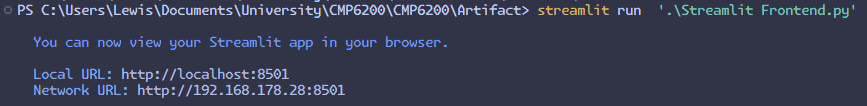
\includegraphics[width=\textwidth]{Artefact/Streamlit/Frontend/CMD.png}
    \caption{Running the chatbot from the terminal with Streamlit. \label{fig:RunApp}}
\end{figure}

\noindent Then, by navigating to the given URL, the chatbot itself can be accessed.

\begin{figure}[H]
    \centering
    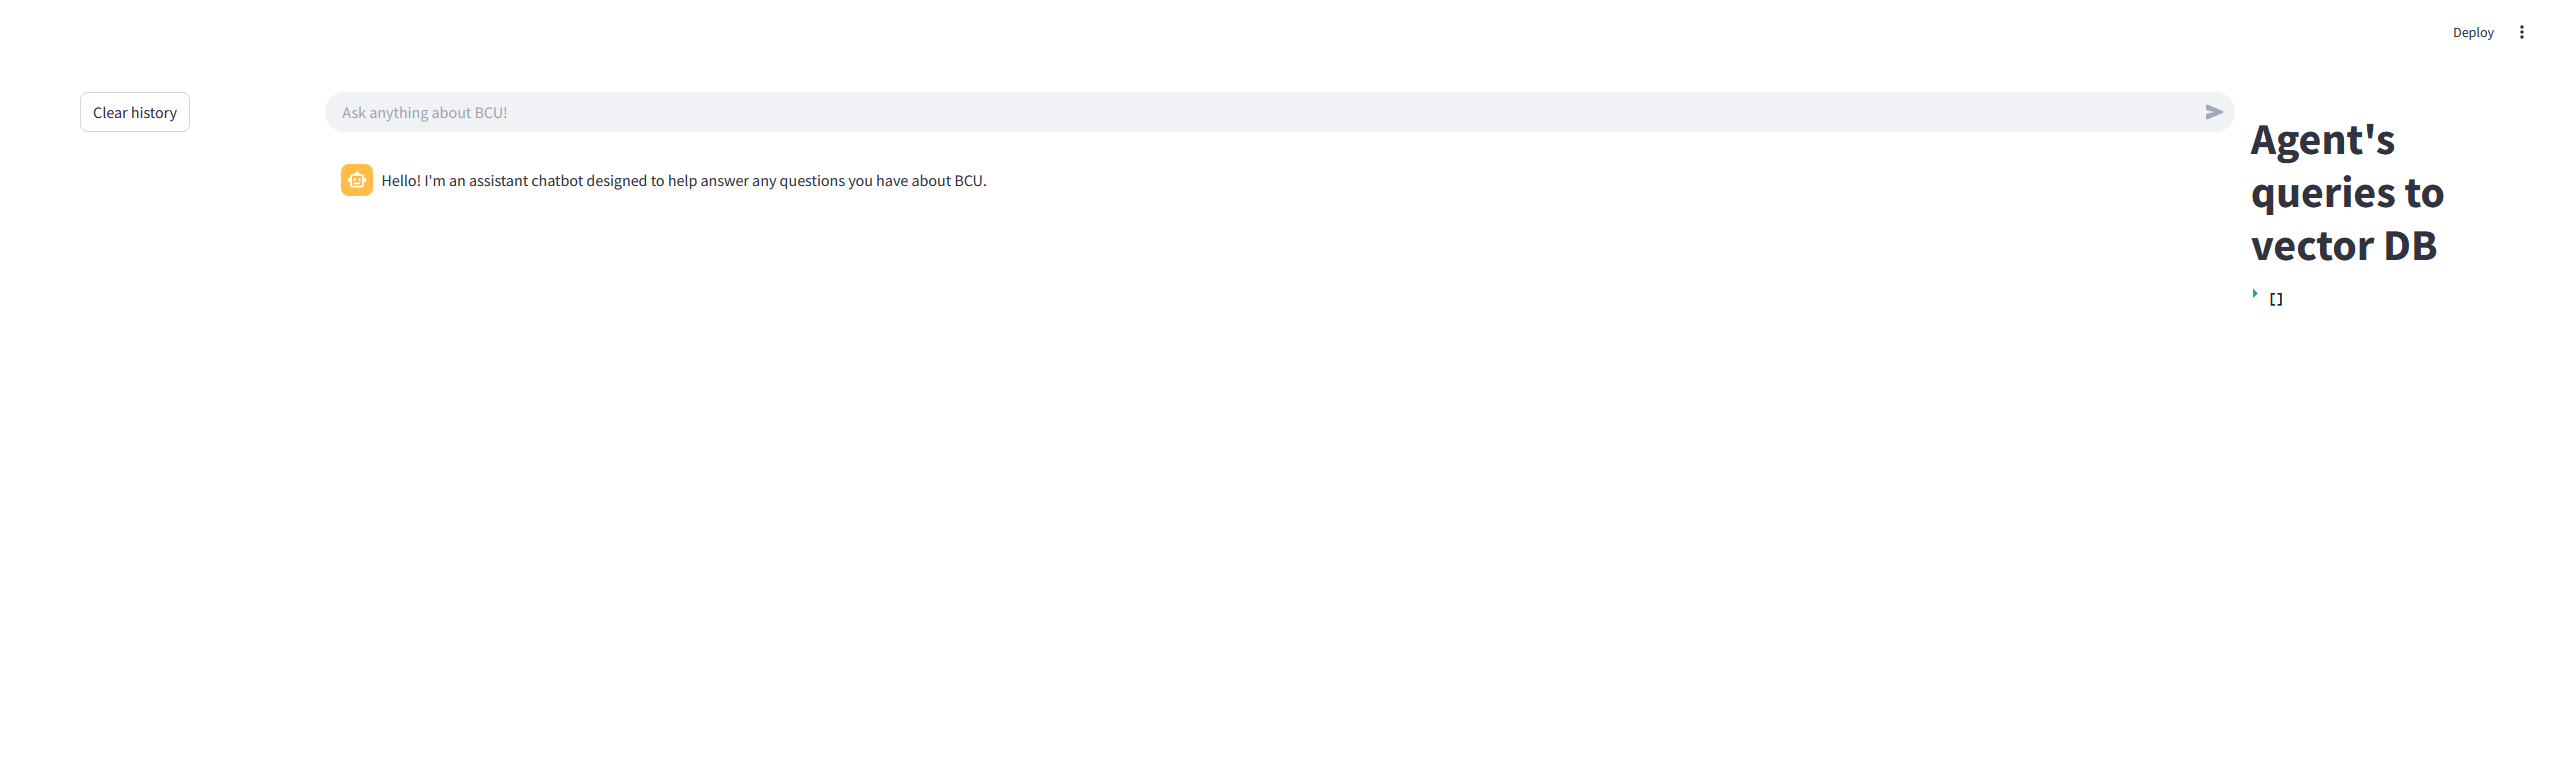
\includegraphics[width=\textwidth]{Artefact/Streamlit/Frontend/FirstRun.png}
    \caption{The chatbot's GUI at its initial state. \label{fig:FirstRun}}
\end{figure}

\noindent The previously defined columns are clearly visible: 'clearHistBtn' as the 'Clear history' button on the left, 'chatHist' as the main 
central column with the text box and default chatbot message, and 'queryLog', currently showing the empty list of queries. 

\para The chatbot can now be queried by simply giving a prompt in the main text entry field as shown in Figure \ref{fig:FirstQuery}, 
which is slightly zoomed in for demonstrative purposes.

\begin{figure}[H]
    \centering
    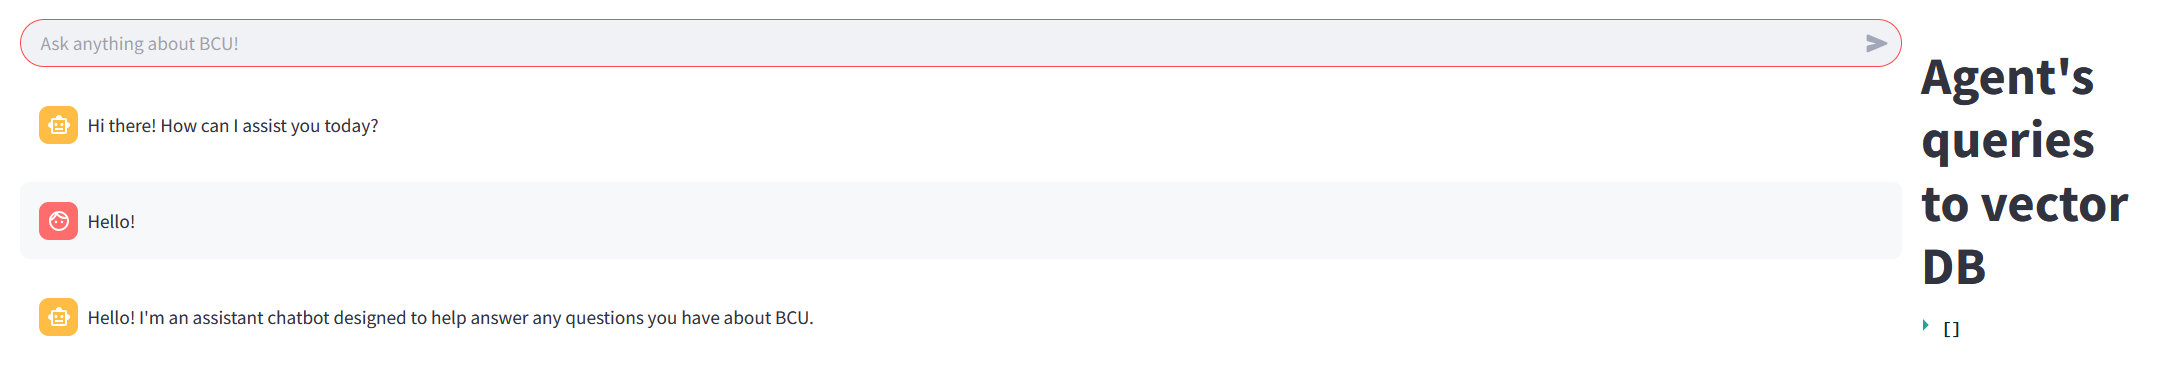
\includegraphics[width=\textwidth]{Artefact/Streamlit/Frontend/FirstQuery.png}
    \caption{Prompting the chatbot with 'Hello!'. \label{fig:FirstQuery}}
\end{figure}

\noindent This simple query demonstrates the conditional branch in LangGraph. With 'Hello' being such a simple query, the chatbot deems 
it unnecessary to retrieve context for, as it can already provide a suitable answer. This can be seen from the 'queryLog' column still 
remaining empty. Instead, the chatbot can now be asked a BCU-related question which it will require context for.

\begin{figure}[H]
    \centering
    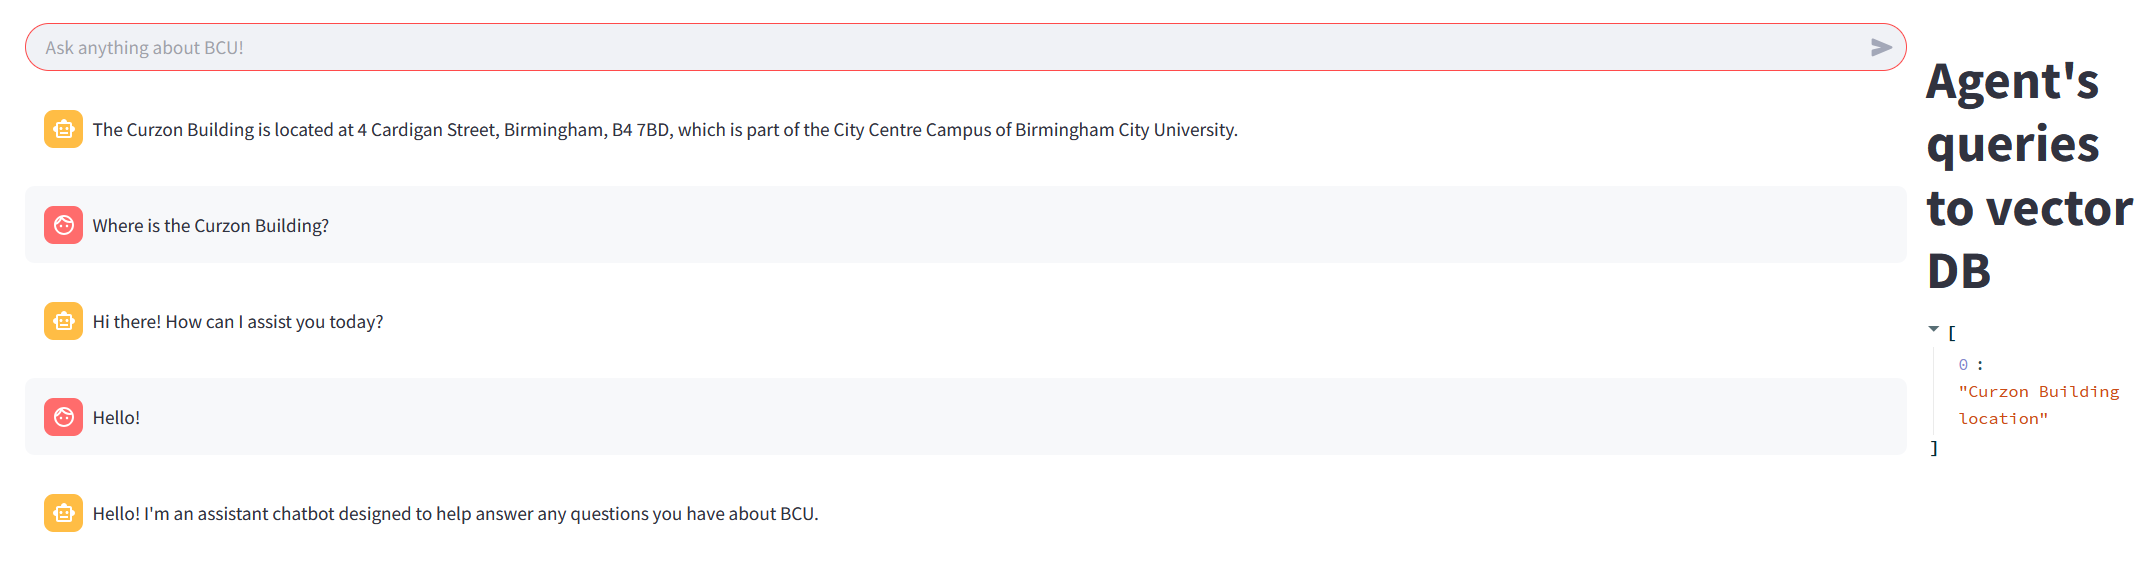
\includegraphics[width=\textwidth]{Artefact/Streamlit/Frontend/SecondQuery.png}
    \caption{Prompting the chatbot with 'Where is the Curzon Building?'. \label{fig:SecondQuery}}
\end{figure}

\noindent The chatbot is able to answer correctly with no hallucination, as it performed a search for 'Curzon Building location' on the 
FAISS database as shown in the 'queryLog' column. From this, it was able to parse the retrieved chunks, locate the address, and return it to the
user. To expand on this functionality, another relevant question can be asked:

\begin{figure}[H]
    \centering
    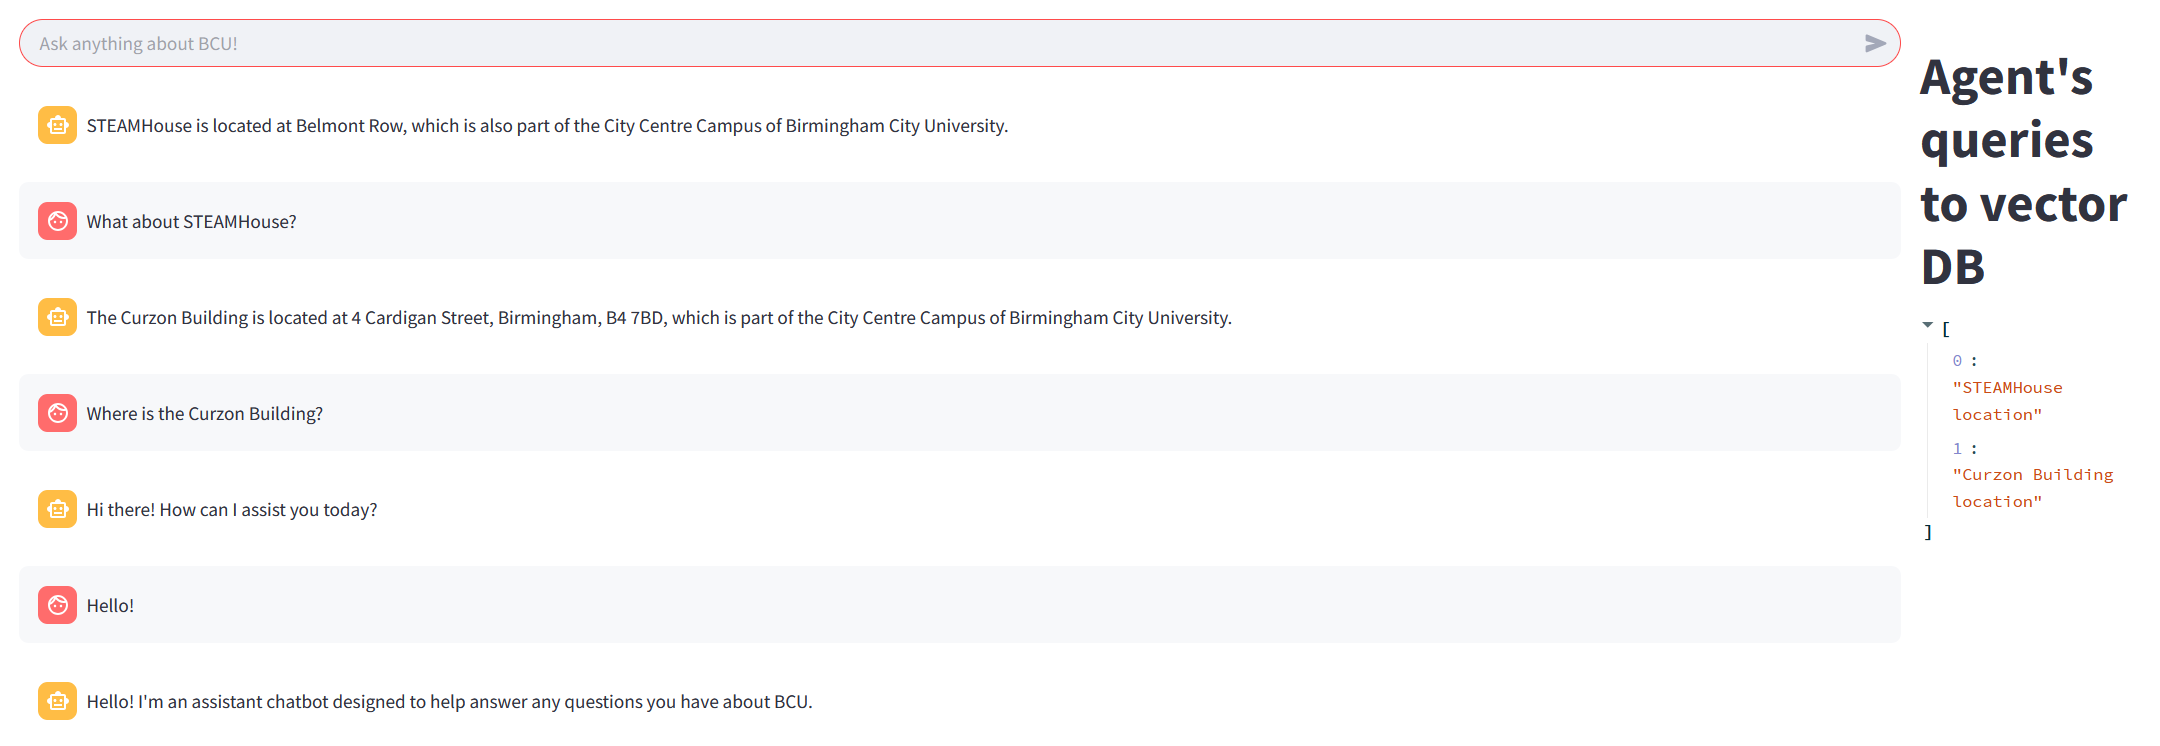
\includegraphics[width=\textwidth]{Artefact/Streamlit/Frontend/ThirdQuery.png}
    \caption{Prompting the chatbot with 'What about STEAMHouse?'. \label{fig:ThirdQuery}}
\end{figure}

\noindent Because the chatbot is invoked with the conversation history, it is able to interpret what the user means by 'What about', 
referring to another building's location. As such, it uses another similar query on the vector database, this time retrieving information 
for the STEAMHouse building, which it is able to successfully return to the user. Additionally, its response states 'which is also part of 
the City Centre Campus', showing that the previous response it gave was factored into its new response, as per the use of 'also'.

\begin{figure}[H]
    \centering
    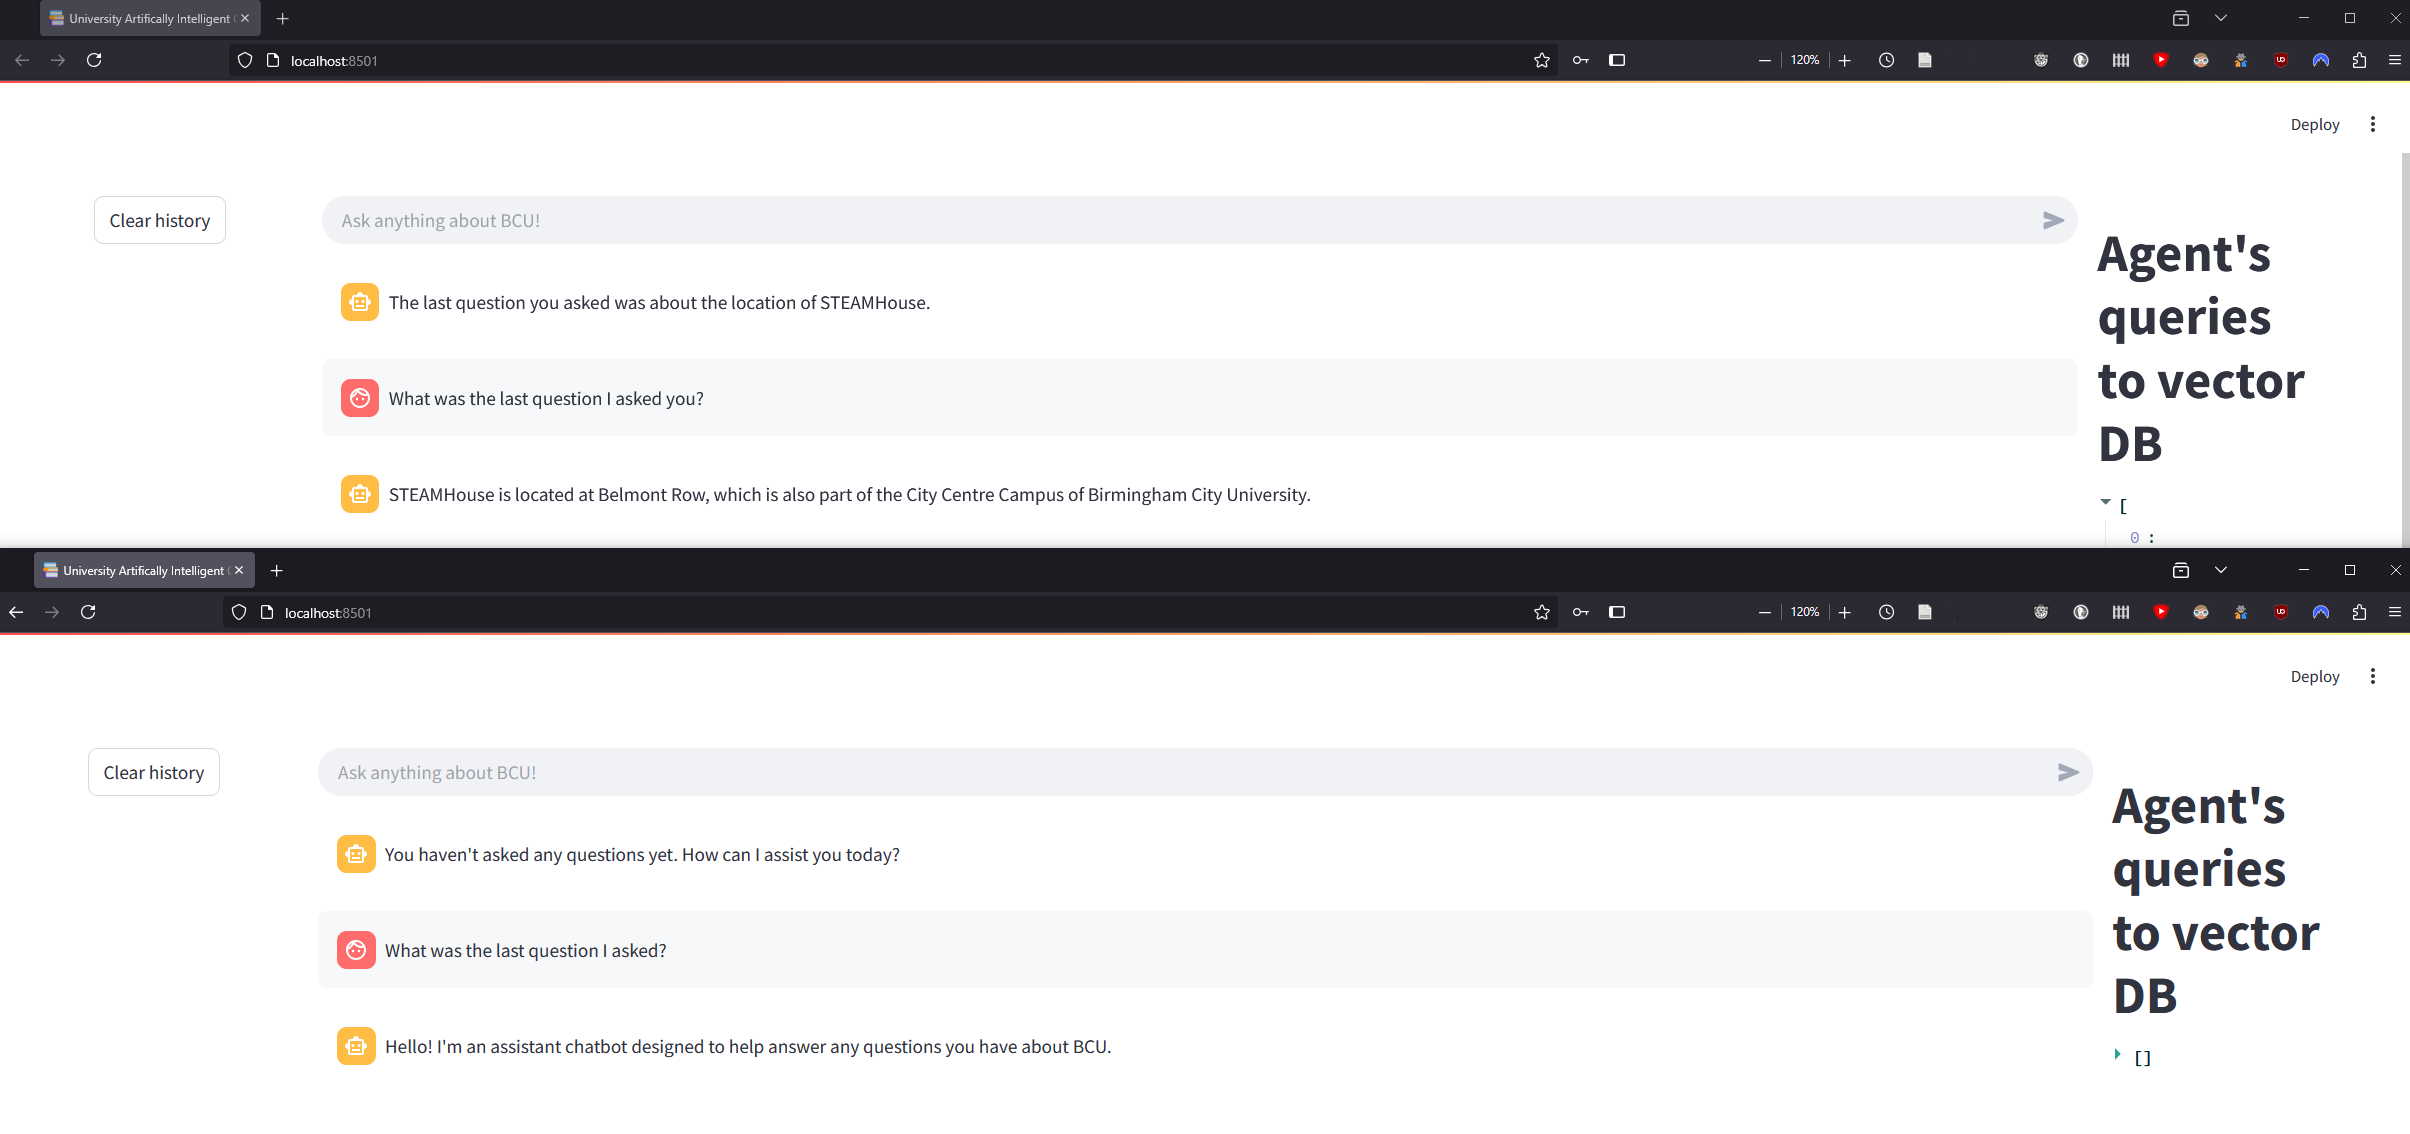
\includegraphics[width=\textwidth]{Artefact/Streamlit/Frontend/UniqueConversations.png}
    \caption{Two separate chatbot instances, which run without memory overlap. \label{fig:UniqueConversations}}
\end{figure}

\noindent Figure \ref{fig:UniqueConversations} depicts how multiple instances of the chatbot can run at the same time without influencing 
each other, which is a key element in terms of user privacy. In the figure, it can be seen that two separate windows of the chatbot are 
running, where one contains the conversation in Figure \ref{fig:ThirdQuery} and another that had just been started. Both chatbots are 
asked what the last question asked of them was, which the new instance cannot answer, but the old instance can. This shows how the second 
chatbot instance runs independently of the first.

% ! What more can really be said? 


    \chapter{Evaluation}\label{ch:Evaluation}
In this chapter, the produced artefact will be evaluated against its original requirements.
In addition, the development process itself will be reflected upon to identify where issues arose 
and could have been prevented.

\section{Methodology}\label{sec:DeepEval}
% Within Section \ref{sec:Requirements}, the functional and non-functional requirements for this project were stated.
% Of these requirements, the chatbot successfully meets all functional requirements, as well as the original aims and 
% objectives stated in \ref{sec:AimsAndObjectives}. However, two non-functional requirements were not met.

% \para One of these requirements was 'The chatbot could allow for voice input and output.' This requirement was not met,
% as it would introduce a significant cost and time investment in trying to integrate this functionality into a Streamlit 
% web app. The other unmet requirement was 'The chatbot could be deployed on an existing messaging service.' This requirement 
% was not met due to time constraints, which is further reflected upon in Section \ref{sec:EvalProcess}. 

\para To properly evaluate the chatbot, it is best to use direct evaluation metrics. While reviewing literature in Section 
\ref{sec:LitReviewLLM}, an evaluation platform known as DeepEval was considered, with the ability to use an LLM as a judge of 
other LLMs \autocite{deepeval_introduction_2024}, known as 'G-Eval'.

DeepEval offers a wide variety of metrics, with one of these metrics being 'GEval'. GEval is a metric which is scored by an LLM based 
on criteria given in natural language, originally created by \textcite{liuGEvalNLGEvaluation2023a}. This means that the metric is directly 
programmable using a system prompt as seen with the chatbot itself.

\para 
To evaluate the chatbot, an evaluation dataset of questions and their expected answers was provided, with the chatbot's actual response being
compared to the expected answer which is known to be true (referred to as a 'golden answer'.). It is common practice when using G-Eval to use a 
superior LLM for evaluation than the one that originally generated the answer. Therefore, for G-Eval, gpt-4o was used, making the evaluation process 
the most expensive part of this project's development cycle. 

\subsection{Dataset and evaluation metrics}

\para Table \ref{tab:GoldenDataset} depicts the golden dataset\footnote{BCU's extenuating circumstances policy was updated during the development of the chatbot to where the fourth question's answer is not entirely correct. However, the chatbot is unaware of this, and the objective was to assess the chatbot's performance against its knowledge base sourced in February 2025, so this is not a major issue.} used to evaluate the chatbot's performance, produced by myself after my own in-depth analysis of each policy in the vector store. 

\begin{longtable}{ | p{0.05\linewidth} | p{0.3\linewidth} | p{0.6\linewidth} | }
    \hline
    \cellcolor{blue!25} ID & \cellcolor{blue!25} Question & \cellcolor{blue!25} Expected answer \\
    \hline
    1 & What happens if I submit my assignment 3 days late? &
    If an assignment is submitted 3 days late, your mark will be reduced by 10\%. \\
    \hline
    2 & What happens if I submit my assignment 3 \textbf{minutes} late? &
    If an assignment is submitted 3 minutes late, it is not considered a late submission, and your mark will not be reduced. \\
    \hline 
    3 & What is an EC claim? &
    An Extenuating Circumstances claim can be made by a student if there are circumstances that affect their ability to submit assessments on time, complete assessments to a good standard or attend in-person assessments. \\
    \hline 
    4 & What circumstances will be accepted as extenuating circumstances? &
    Serious short-term illness or injury, worsening of an ongoing illness or disability, symptoms of a harmful infectious disease, death or significant illness of a close family member or friend, unexpected caring responsibilities, significant personal or family crises, witnessing or experiencing a traumatic incident, a crime which has had a substantial impact on you, an accommodation crisis such as eviction.\\
    \hline 
    5 & When must I enrol? & 
    Students must enrol at the start of their programme and enrol for each level by the Friday of week four from the start date of their course unless a Break in Study has been approved. \\
    \hline 
    6 & What is the pass mark for a module? &
    For an undergraduate course, the pass mark is 40\%. On a postgraduate course, it is instead 50\%. \\
    \hline 
    7 & What happens if I fail a module? &
    The first time you fail a module, you can be re-assessed for failed assessments, which is known as a resit. Your grade will be capped at the pass mark. You cannot be reassessed for assessments that you passed. \\ 
    \hline 
    8 & What are the degree classifications? &
    Achieving an average of 70\% or above grants you first-class honours. 60-69\% is an upper second (2:1), 50-59\% is a lower second (2:2), 40-49\% is third-class honours, and anything below 40\% is a fail. \\
    \hline 
    9 & How many BCU students are there? &
    BCU has 31,300 students as of 2022-23. \\ 
    \hline 
    10 & What is BCUSU? &
    The Birmingham City University Student Union represent you as a student, and work together with the university to make change. They can help with various academic topics and offer societies to help people make friends. \\
    \hline
    \caption{The golden dataset for chatbot evaluation.}\label{tab:GoldenDataset}
\end{longtable}

\para The golden dataset was then stored as a nested array of question/answer pairs where for each item in the array, index 0 was the question 
and index 1 was its respective answer. 

\begin{figure}[H]
    \centering
    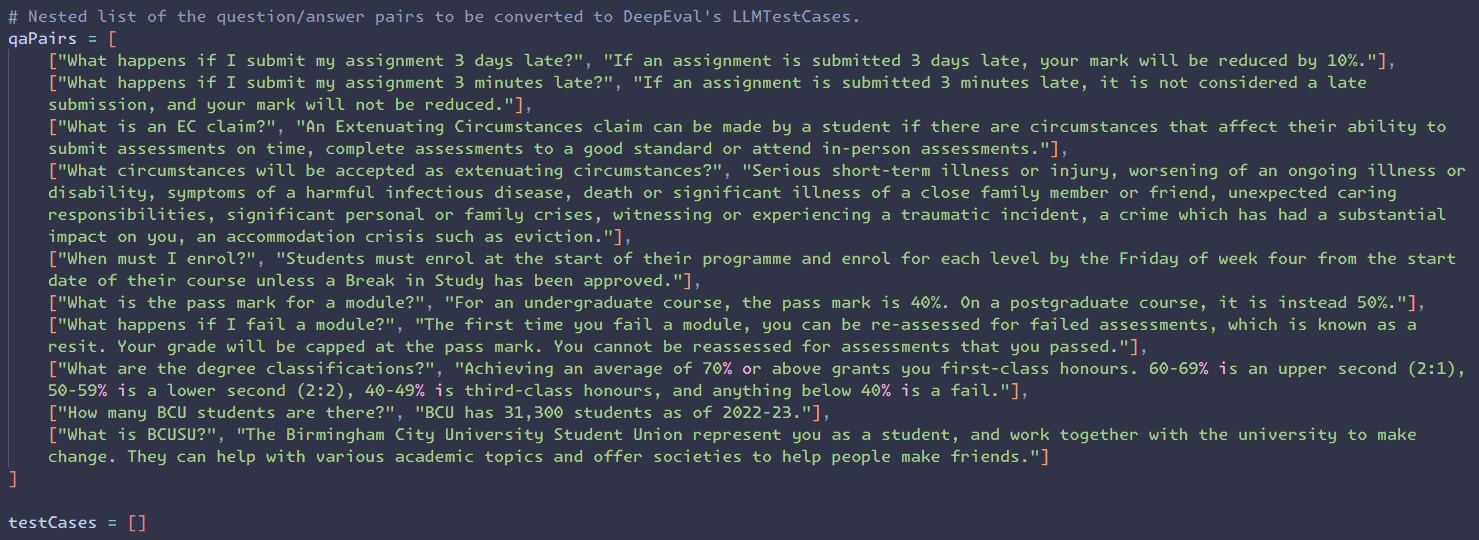
\includegraphics[width=\textwidth]{Evaluation/QAPairs.png}
    \caption{The golden dataset as represented in the evaluation script. \label{fig:GoldenDataset}}
\end{figure}

These question/answer pairs were then used to generate DeepEval's own 'LLMTestCase' classes for each item, 
with the input being the question, expected output being the golden answer, and the actual output using the 
testChatbot function to invoke the chatbot.

\begin{figure}[H]
    \centering
    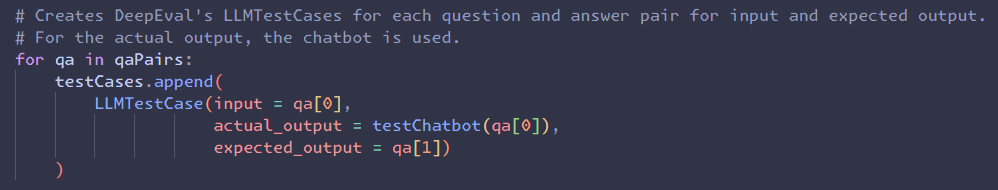
\includegraphics[width=\textwidth]{Evaluation/CreateTestCases.png}
    \caption{Iteratively creating DeepEval LLMTestCases for each question/answer pair. \label{fig:CreateTestCases}}
\end{figure}

\para The test cases were then added into a DeepEval 'EvaluationDataset' for later use. Then, the GEval metric was defined.

\begin{figure}[H]
    \centering
    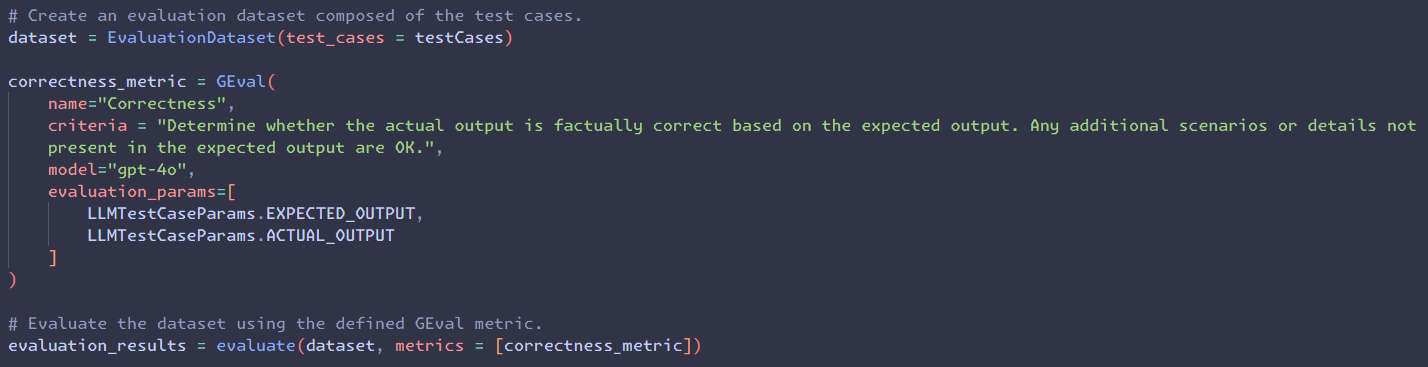
\includegraphics[width=\textwidth]{Evaluation/GEvalMetric.png}
    \caption{Creating the evaluation dataset and GEval metric. \label{fig:GEvalAndDataset}}
\end{figure}

\noindent The criteria field of the GEval metric acts as the system prompt for the gpt-4o model. In the criteria, the LLM is told 
to evaluate the 'correctness' of the actual output by comparing it against the expected output. An additional note was added to ensure 
that the chatbot was not penalised for giving more information than strictly necessary, as GEval would originally fail some test cases 
as the actual output was sometimes too informative compared to the expected output.

\para Following all of these initial steps, the primary DeepEval 'evaluate' function is called using the created EvaluationDataset
and GEval metric. 

\section{Baseline systems}
Multiple vector stores were created for the chatbot, each using a differing chunk size and overlap. A total of four datasets were 
made, all of which used FAISS as the backend engine and PyPDFLoader to load each PDF prior to chunking. 

\para These vector stores were:
\begin{itemize}
    \item FAISS \begin{itemize}
        \item The original vector store used throughout early development.
        \item Chunk size: 1000
        \item Overlap: 200
    \end{itemize}
    \item FAISS-SmallChunks \begin{itemize}
        \item As suggested by its name, used a lower chunk size and overlap than others.
        \item Chunk size: 500
        \item Overlap: 100 
    \end{itemize}
    \item FAISS-BigChunks \begin{itemize}
        \item Used bigger chunks and overlap than the original vector store.
        \item Chunk size: 1500
        \item Overlap: 300
    \end{itemize}
    \item FAISS-HugeChunks \begin{itemize}
        \item The vector store used in the final product.
        \item Chunk size: 2000
        \item Overlap: 500
    \end{itemize}
\end{itemize} 
    \section{Results}

\begin{figure}[H]
    \centering
    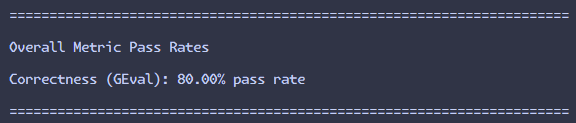
\includegraphics[width=\textwidth]{Evaluation/FAISS-HugeChunks/Overall.png}
    \caption{Overall GEval results against the "FAISS-HugeChunks" vector store (80\% correctness against expected outputs) \label{fig:EvalResults}}
\end{figure}

\noindent On the ten test cases on various academic policies and information used in evaluating the chatbot,
80\% were answered correctly according to GEval. Figures \ref{fig:WrongAnswer1} and \ref{fig:WrongAnswer2} depict 
the two queries where the chatbot failed to give a suitable answer.

\begin{figure}[H]
    \centering
    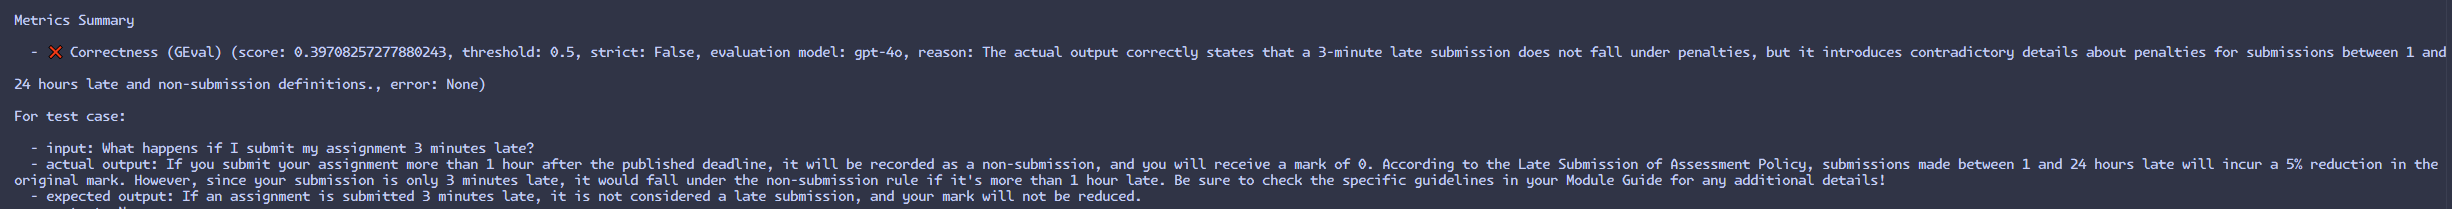
\includegraphics[width=\textwidth]{Evaluation/FAISS-HugeChunks/Incorrect1.png}
    \caption{The first incorrect answer, with the chatbot answering incorrectly. \label{fig:WrongAnswer1}}
\end{figure}

\noindent This question was answered incorrectly due to the chatbot's misinterpretation of the related policy. Work submitted up to 
1 hour after a deadline does \textbf{not} receive any grade penalty, though the chatbot likely read the following sentence: work submitted between 1 hour and 
24 hours after a deadline \textbf{does} incur a penalty. As such, this misinterpretation lead to the question being answered incorrectly.

\begin{figure}[H]
    \centering
    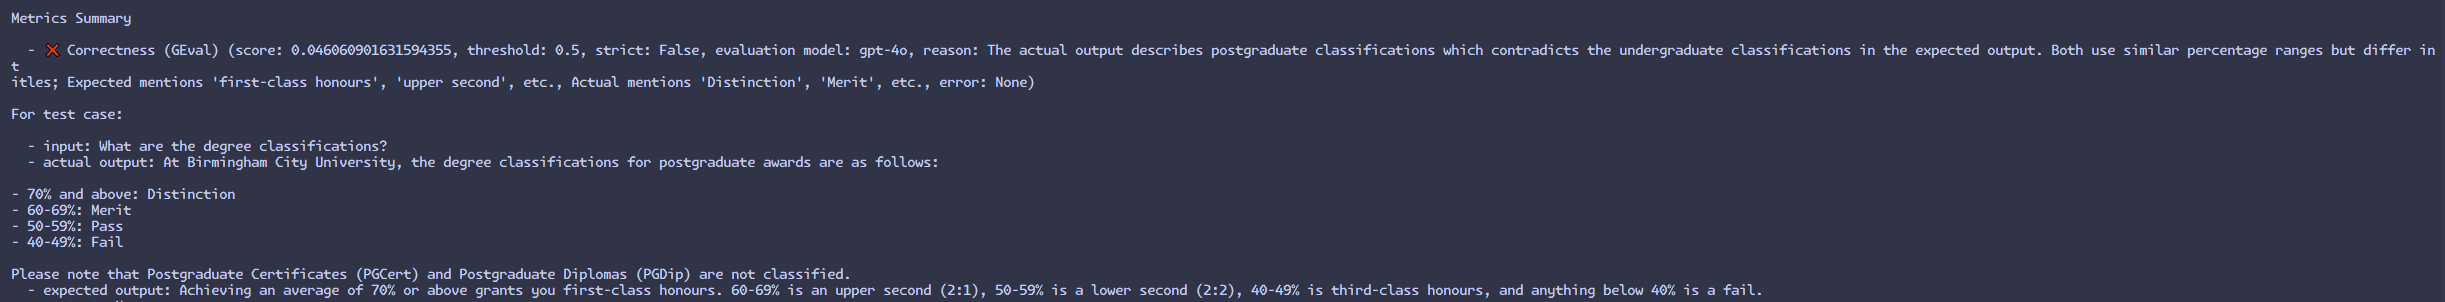
\includegraphics[width=\textwidth]{Evaluation/FAISS-HugeChunks/Incorrect2.png}
    \caption{The second incorrect answer, with incorrect information retrieval. \label{fig:WrongAnswer2}}
\end{figure}

\noindent The chatbot retrieving information that isn't directly relevant for this question implies an error in the retrieval tool. 
This could likely be due to the format of each policy document, with the information requested here (degree thresholds) being stored in
a table, depicted in Figure \ref{fig:WrongAnswer2Snippet}.

\begin{figure}[H]
    \centering
    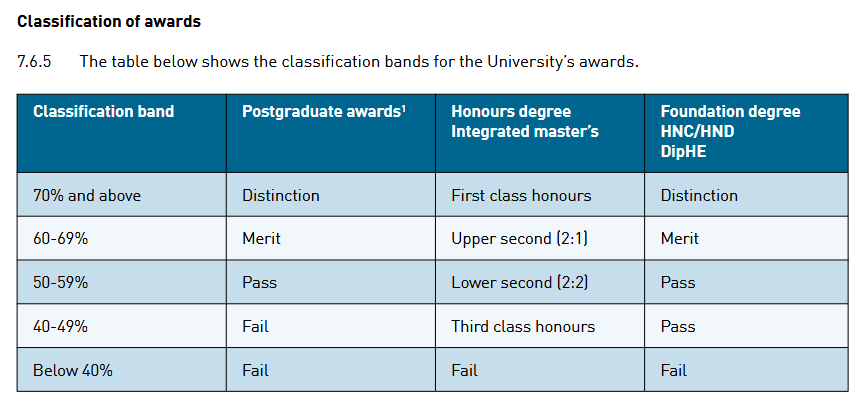
\includegraphics[width=\textwidth]{Evaluation/WrongAnswerPolicy.png}
    \caption{The snippet of the Academic Regulations that should have been referenced. \autocite{bcuPoliciesProcedures} \label{fig:WrongAnswer2Snippet}}
\end{figure}

\noindent The 'PyPDFLoader' class in LangChain, which was used when storing all University data, can sometimes misinterpret tables. 
This may in turn have created issues with the semantic search performed on the FAISS DB, leading to this question going unanswered as 
the search was unable to identify each degree classification.


\subsection{Functional requirements} 
The functional requirements, and how they were met, were as follows:

\begin{itemize}
    \item The chatbot must interpret and respond to answers in English.
    \begin{itemize}
        \item This requirement was fully met with no particular involvement from myself. OpenAI's models can automatically 
        interpret and respond with English text, as well as other languages, though other languages were not tested as I 
        cannot verify them. 
    \end{itemize}
    \item The chatbot must accept text queries.
    \begin{itemize}
        \item This was automatically met through the use of OpenAI models.
    \end{itemize}
    \item The chatbot must respond using text.
    \begin{itemize}
        \item This was automatically met through the use of OpenAI models.
    \end{itemize}
    \item The chatbot must be accessible at all times.
    \begin{itemize}
        \item When the Streamlit application is running, the chatbot can always be accessed 
        by any device connected to the same network, as long as they connect with the IP and port
        which Streamlit specifies.
    \end{itemize}
    \item The chatbot must supply BCU-related information.
    \begin{itemize}
        \item A vector database using FAISS was created containing a wide variety of BCU policies and miscellaneous
        information. Using this database, the chatbot had access to a retrieval tool which would perform a semantic 
        search on the database to retrieve BCU information relating to the user's query.
    \end{itemize}
    \item The chatbot must answer at least 75\% of BCU-related queries correctly.
    \begin{itemize}
        \item GEval reported an accuracy of 80\% against the manually produced golden answers. This is over 75\%,
        though perhaps not by a satisfactory amount. A larger testing dataset will help to provide a more accurate 
        picture in future.
    \end{itemize}
    \item The chatbot must have a GUI for ease of use and accessibility.
    \begin{itemize}
        \item Streamlit acts as the chatbot's frontend, providing a responsive and sleek UI that adapts to 
        desktop web browsers and mobile devices. The UI is simple to understand and can be navigated with the 
        Tab key on a keyboard for people unable to use a mouse.
    \end{itemize}
    \item Multiple users must be able to use the chatbot at the same time.
    \begin{itemize}
        \item Streamlit facilitates this functionality, creating isolated instances of the chatbot which do not interact 
        with each other.
    \end{itemize}
\end{itemize}

\noindent All functional requirements of the chatbot's original scope were met, producing a usable product which students 
can use to get BCU-related information at a satisfactory level of accuracy. 

\subsection{Non-functional requirements}
The non-functional requirements, and how they were met (or failed to be met) are as follows:

\begin{itemize}
    \item The chatbot should respond to queries within 10 seconds.
    \begin{itemize}
        \item All conversations with the chatbot throughout testing would gather responses 
        in fewer than 10 seconds. Queries that used RAG took significantly longer than those which 
        did not. The overall 'feel' of the app could be made faster by allowing the LLM to stream 
        text rather than output a full message, which will show the message being procedurally written 
        rather than a buffer before a full message suddenly appears.
    \end{itemize}
    \item The chatbot could allow for voice input and output.
    \begin{itemize}
        \item This requirement \textbf{was not met.} This was mostly due to time constraints, as implementing this 
        functionality would have taken substantial research that would likely not have been possible to perform 
        while meeting project deadlines. Unfortunately, this does make the app less accessible, forcing users 
        to be able to use a keyboard or have third-party voice software to input text.
    \end{itemize}
    \item The chatbot could be deployed on an existing messaging service such as Teams.
    \begin{itemize}
        \item This requirement \textbf{was not met.} As with the voice requirement, this would have taken additional 
        research and a possible redesign of the app's backend to provide an API compatible with a messaging 
        service chatbot. Given that Streamlit already provides a usable and modern UI, this requirement was instead 
        considered unnecessary.
    \end{itemize}
\end{itemize}

\noindent Only one of the three non-functional requirements was met due to time constraints which plagued development.
Even without the implementation of these features, however, the chatbot is still a very usable product. 
    \section{Discussion}

\subsection{Accomplishments}
Overall, it is safe to say that the project can be considered a success, though it certainly is not without flaw.
It was previously mentioned that the chatbot had an accuracy of 80\% according to GEval, though this was only against a dataset 
of 10 questions. It would be much more suitable to expand this training dataset, alongside gathering actual user feedback.

\para Additionally, my own limitations in knowledge when it came to LangChain and LangGraph meant that I was unable to optimally refine the 
retrieval tool to work on the failed questions in time, and I was also unable to successfully implement a ReAct agent as researched in the 
literature review.

\para Despite the project's few failures, there was a greater amount of successes. I have hugely increased my own knowledge of Python, LLMs,
and RAG. These are three critical skills to have if I intend to work in software development due to recent trends with companies 
becoming more reliant on LLMs. 

\para Furthermore, through developing the chatbot and performing the extensive research required, I believe my skills as an overall software 
developer have enhanced in a way that is not exclusive to Python; I have become much more aware of how to interpret API references and documentation,
meaning that my ability to adapt to new tech stacks as seen in this project should now be a much faster process.

\para The achievement I am most proud of with the chatbot is the cost-saving effort of the conditional branches. Originally, the chatbot would 
query the database for every prompt given, even if it was something as simple as 'Hello!'. This would lead to 6,000 characters worth of university
data which would not be relevant to the query being given to the LLM, wasting processing time and money through the greatly increased token cost 
of such a prompt, as well as resulting in a strange and irrelevant response that would only serve to confuse the user. 

\section{Development process}\label{sec:EvalProcess}
\subsection{Positives}
All functional requirements stated in Section \ref{sec:Requirements} for the final product, as well as the original aims and objectives 
of the project, were successfully met with a working chatbot with good accuracy on BCU-related topics being produced in a timely fashion.

\para Furthermore, with the project being a solo endeavour, a comprehensive understanding of the project management life cycle was 
obtained from conception to completion. As a result, I believe my problem-solving and decision-making skills have greatly improved.   

\subsection{Negatives}
As identified previously in Section \ref{sec:Limitations}, the most significant limitation throughout the development process 
was the amount of time available. Over the course of the project's development, significant extenuating circumstances occurred 
leading to the lack of some desired features and lower quality of others. Furthermore, balancing the production of this project 
alongside four other university modules simultaneously proved to be an arduous task that I was unable to efficiently solve to 
a level I would have preferred.

\para Cost proved to be a much lesser restriction than initially anticipated, due to the cost efficiency 
provided through the identification of OpenAI's lower-end models through thorough research. 

\para However, the other limitations specified in Section \ref{sec:Limitations} also played key roles of their own, though less significant 
than the time restrictions. Most notably of these was my own lack of experience with LLMs. Developing a product using a tech stack 
I was entirely unfamiliar with prior to development proved to be highly difficult. 

\chapter{Conclusions}
% \textbf{"You should not include any new information or discussion in this section."}
% This section must also link to the project's objectives.

\begin{tcolorbox}[colback=red!5!white,colframe=red!75!black,title=Not present in draft]
    I haven't been able to write this section due to deadline clashes and time constraints.
\end{tcolorbox} 
\chapter{Recommendations for future work}
Lorem ipsum dolor sit amet, consectetur adipiscing elit. Curabitur et erat consectetur, 
scelerisque eros nec, ultricies est. Donec mi ipsum, imperdiet vitae arcu quis, luctus venenatis quam. 
Integer ac massa a augue venenatis fringilla. Etiam posuere libero sed nulla tristique volutpat.


% ! If a reference doesn't have a keyword, it won't show in the bibliography.
% ! Go over the .bib files, ensuring they use a keyword on each reference.

% ? Prevents bibliography overflowing hbox at the expense of it taking up more lines on the page.
\emergencystretch=1.5em
\addcontentsline{toc}{chapter}{References}
\printbibliography[keyword={refs}, title = {References}]


\printbibliography[keyword={bib}, title = {Bibliography}]
\addcontentsline{toc}{chapter}{Bibliography}

\end{document}